\chapter{Data acquisition software}
\label{chapter:dqm4hep}

\epigraph{Before software can be reusable \\it first has to be usable.}{Ralph Johnson}

This chapter will discuss the usage of online monitoring and data quality monitoring software for high energy physics testbeams, specifically the \acrshort{DQM4hep} tool. This tool was initially developed for a specific detector prototype, but was able to be expanded for the use of other detectors. This online monitor was then proposed as an option for Work Package 5 of the \acrshort{AIDA}-2020 collaboration, to be used as a generic online monitor and data quality monitor.

This chapter describes \acrshort{DQM4hep} in detail, including the motivation for the usage of generic software tools as outlined by the \acrshort{AIDA}-2020 collaboration. The codebase, structure, networking and implementation of the software framework is described in detail.

Following this, detailed documentation for a user guide describing the structure, usage, running and authoring of the user-specific parts of the framework is presented. This represented the distillation of significant experience using the framework on many testbeams of different kinds and goals.

This work was presented at the Beam Telescopes and Test Beams workshop in 2016, and was presented as a poster and corresponding conference proceedings at both the Topical Workshop for Electronics in Particle Physics\cite{dqm4hep-twepp} and the \acrshort{IEEE} Nuclear Science Symposium and Medical Imaging Conference\cite{dqm4hep-ieee} in 2017. In addition, I led a software training session in the use of \acrshort{DQM4hep} at the Beam Telescopes and Test Beams workshop in 2017. % Feels weird to say "I" here

\section{Introduction}
\acrfull{DAQ} is a critical component of all modern particle physics experiments across all stages of technological readiness, from the very beginning of hardware testing in tabletop experiments to full-scale international experiments like the Large Hadron Collider.

In the modern era of particle physics, the interplay of hardware and software at minuscule timescales drives everything, and almost all results are highly dependent upon the speed and efficiency of the electronics and computer systems that extract data from the detectors. A massive quantity of work goes into creating, testing and optimising the systems that will acquire, process, sort and transport data before it is ever seen by the physicist operating the experiment.

Of particular interest in this thesis is the data acquisition software during the development phase, where individual detector subcomponents are undergoing prototyping and testing. These development and iteration cycles are tied closely to testbeam facilities such as the \acrfull{SPS} at \acrshort{CERN} and the DESY II synchrotron at \acrshort{DESY}. At this point in the development cycle, the detectors are beginning to take shape and this is where data acquisition (or \acrshort{DAQ}) becomes an important consideration. 

In addition to this, the data acquisition solutions used during the testbeam phase of detector development is likely to inform the final data acquisition solution; either by evolving directly into the final software, or by identifying and evaluating the particular features or challenges of the subdetector components that the software must take into account or accommodate.

During this stage, each individual detector component -- such as a vertex tracker or hadronic calorimeter -- will be developed by small teams, and the natural tendency is for each of these groups to set their own standards and develop their own tools, prioritising the features that are important to their specific case. However, in the past this approach has generated a variety of \textit{ad hoc} solutions for testbeam software, many of which cannot be applied outside of their original scope. This results in different teams solving the same problems and implementing the same solutions for each subdetector.

An alternative to this is to develop a suite of tools or frameworks that are generic -- capable of being used and deployed for a wide variety of different uses and detector types. In this way, we could greatly reduce the effort used to recreate the same solutions for each new detector, allowing more science to be done faster.

\subsection{Online monitoring and data quality monitoring}
The area of this that we have chosen to contribute to is the development of online monitoring and data quality monitoring tools. Data from testbeams is often not processed fully until well after it has been taken, sometimes after the testbeam has ended, due to constraints on time or processing power. If there were errors, incongruencies, or any other issues with the data, these issues cannot be identified immediately, and as a result may be present in multiple runs, spoiling data and wasting precious time during the already extremely time-sensitive environment of a testbeam.

Online monitoring addresses these issues by allowing the experimenters to see a ``preview'' of the data being collected. It can provide both a quantitative and qualitative look into how the detectors are responding, and what the data will look like when properly processed, allowing any potential issues to be identified and fixed in a timely manner. This means that good online monitoring can improve the efficiency of a testbeam, increasing the ``yield'' of data from a given experiment.

Another aspect of this is data quality monitoring (\acrshort{DQM}), which assesses the `quality' of the data being taken. The definition of data's `quality' will vary depending on the hardware, software, and goals of the experiment, but will usually constitute a some from of statistical measure. In this regard, data quality monitoring can be seen as an extension of the concept of online monitoring, focusing more closely on the quantitative aspects. In general, \acrshort{DQM} provides the most benefit in more mature experiments, relying on previous experience with the detector and collected data to understand how the data appears when the device is functioning correctly.  

In pursuit of all of the above aims, this chapter will discuss the \acrlong{DQM4hep} tool (\acrshort{DQM4hep}) developed for online monitoring and data quality monitoring, going into detail on its properties, principles, applications and development. Deployment and usage of the framework will be discussed in greater detail in Chapters \ref{chapter:aidatestbeams} and \ref{chapter:ideatestbeam}.

\subsection{The \acrshort{AIDA}-2020 project}
This work on \acrshort{DQM4hep} takes place within the context of the \acrshort{AIDA}-2020 project \cite{aida-2020} , an EU-funded research programme for developing infrastructure and technologies for particle physics detector development and testing, comprising 24 member countries and lead by \acrshort{CERN}.

The overarching goal of \acrshort{AIDA}-2020 is to develop common tools and infrastructures for physics testbeams. The collaboration is split into work packages focusing on specific areas, and the work detailed in this thesis takes place within Work Package 5 for data acquisition systems for beam tests.

The goal of this work package is to create a suite of tools that are designed with a variety of possible uses in mind, thereby reducing the work and development time necessary to implement data acquisition and monitoring setups, speeding up the planning and deployment of physics testbeams. 

\section{Overview of DQM4hep}
Data Quality Monitoring for High-Energy Physics (abbreviated \acrshort{DQM4hep}) is an online monitoring and data quality monitoring framework developed for physics testbeams for high-energy and particle physics, developed by R\'{e}mi Et\'{e} and Antoine Pingault. It is designed to be able to fulfil the requirements of monitoring for physics testbeams in a generic way. The framework is written in the C++11 standard and can run on any Linux distribution. The only requirements for installation are a compiler compliant with the C++11 standard, cmake 3.4 or higher, and ROOT 6. All other dependencies are downloaded and compiled automatically during installation. 

The two core principles of \acrshort{DQM4hep} are genericness and modularity. The framework is based upon a plugin system that allows shared libraries to be loaded and hook classes for further use \cite{aida2020-milestone-dqm4hep}. This structure allows for independent components of the framework to be used, not used, or exchanged, by isolating each function of the program into independent processes. The components that are specific to any particular use case are written by the users, and the rest of the framework then handles packaging this information in a useful way and networking to transmit it to where it is needed, meaning that the user does not have to worry about the mechanics of data storage, serialisation or transmission. 

The experiment-specific components have to be written by the user, but these components use standard C++ code with a few \acrshort{DQM4hep}-specific functions to handle their integration into the framework, making them easy to understand for users who already have experience coding in C++. This also means that the framework is capable of working with any data format that can packed into, decoded from, and accessed with normal C++ methods, including those that can be loaded from external libraries. This results in a framework that is able to deal with any kind of data, including user-defined data types, making it more flexible, portable and easily reusable.

\subsection{Architecture}
\acrshort{DQM4hep} is designed with genericness as its core paradigm, using processes and algorithms that are independent of data type. The ability to run multiple instances of each process of the framework is also key to its flexibility, allowing users to, for example, separate sub-detector data from data that has undergone event building, operate in online or offline modes, or distribute the computational load of the analysis over several networked computers.

The generic nature of the framework lies in two core features:

Firstly, the abstract \acrfull{EDM}. An event data model is the structure of the events in the data. For instance, a software `event' might in fact be a readout cycle, where the detector writes data to the data acquisition device when its memory is full. Or it might be a physical event, in which case the event is further defined by the trigger -- an event that is triggered internally by the detector itself will have a different structure to an event that is externally triggered, such as by a bunch-crossing ID. \acrshort{DQM4hep} uses an abstract container for the event itself and allows the user to define its type, structure, and how serialisation should be handled. This means it can handle \textit{any} type of data.

Second, the plugin system. This is a system that allows the inclusion of any user-defined classes or methods via external libraries. These can be used to specify the serialisation method for data, the procedure for online analysis, or many other purposes. 

The plugin system for end-users consists of four different types of plugins: analysis modules, standalone modules, file reader plugins, and file streamer plugins. Each of these will be discussed in-depth in the sections below.

A diagram of the overall structure of the framework can be seen in Fig. \ref{figure:daq/dqm4hep/architecture}.

\begin{figure}[p]
	\centering
	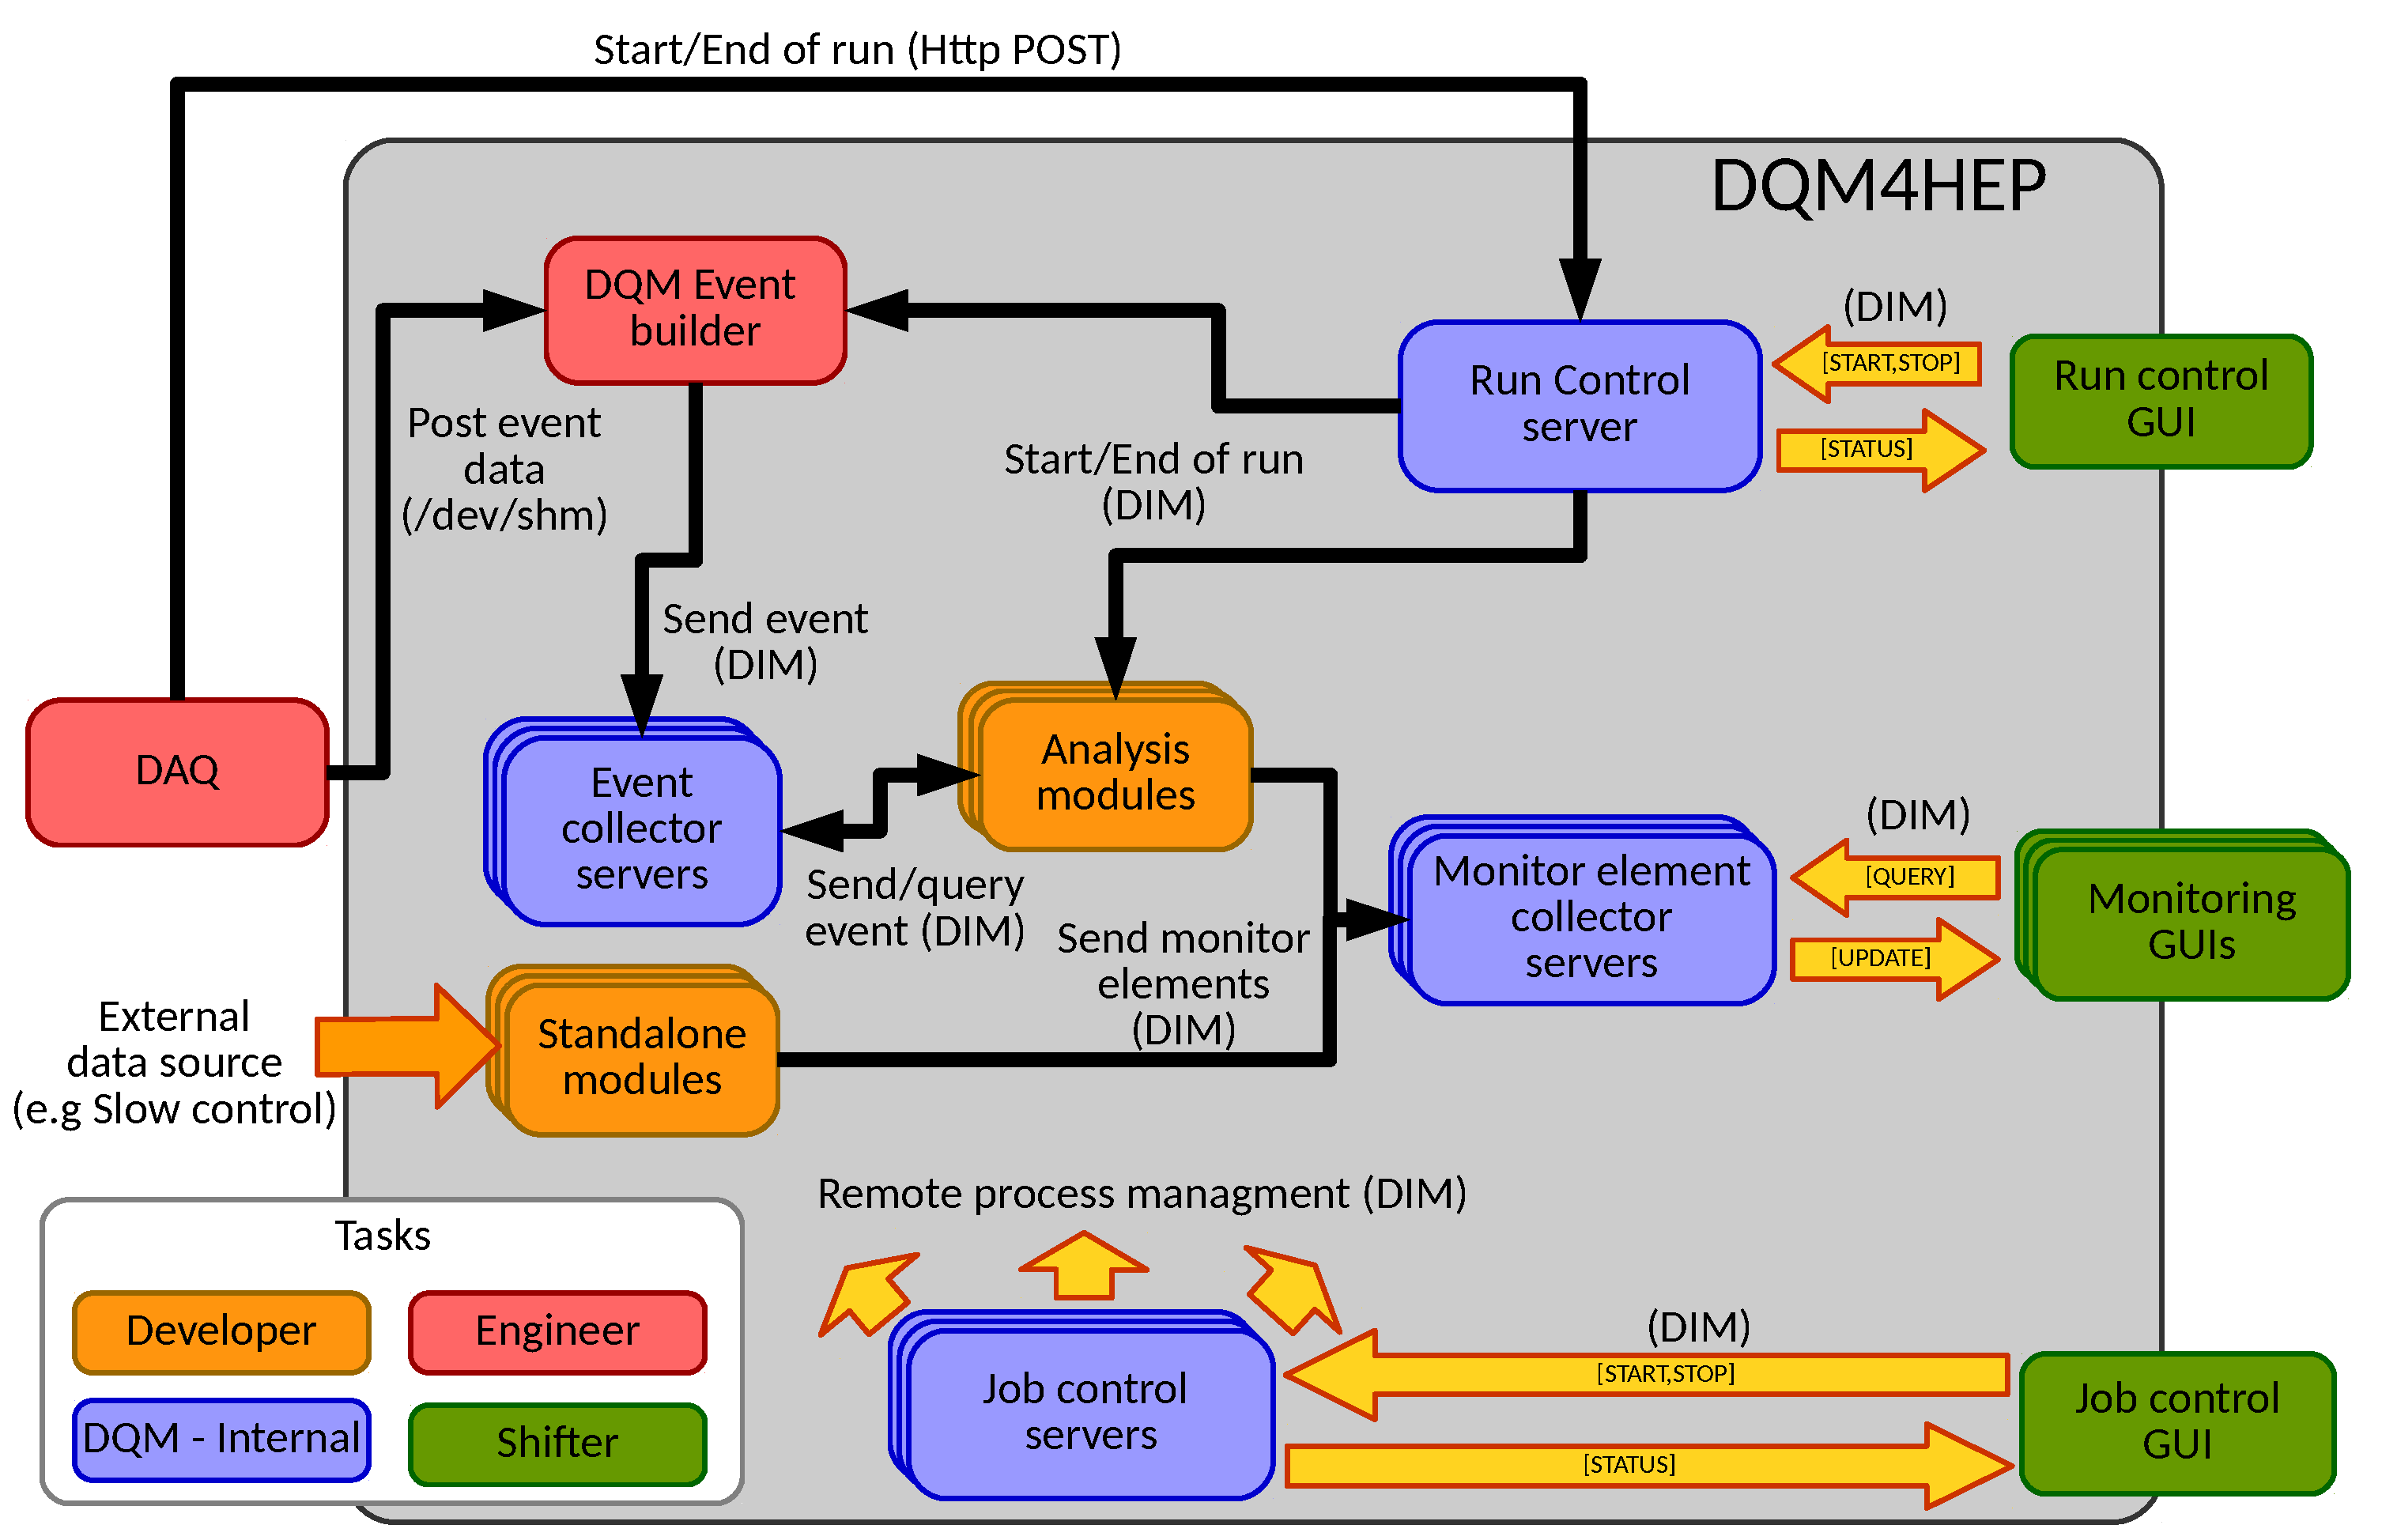
\includegraphics[width=0.95\textwidth]{../Pictures/GlobalArchitectureDiagram.pdf}
	\caption{The global online architecture of \acrshort{DQM4hep}. Each block is colour-coded to show which operator of the testbeam is responsible for the process.}
	\label{figure:daq/dqm4hep/architecture}
\end{figure}

\begin{figure}[p]
	\centering
	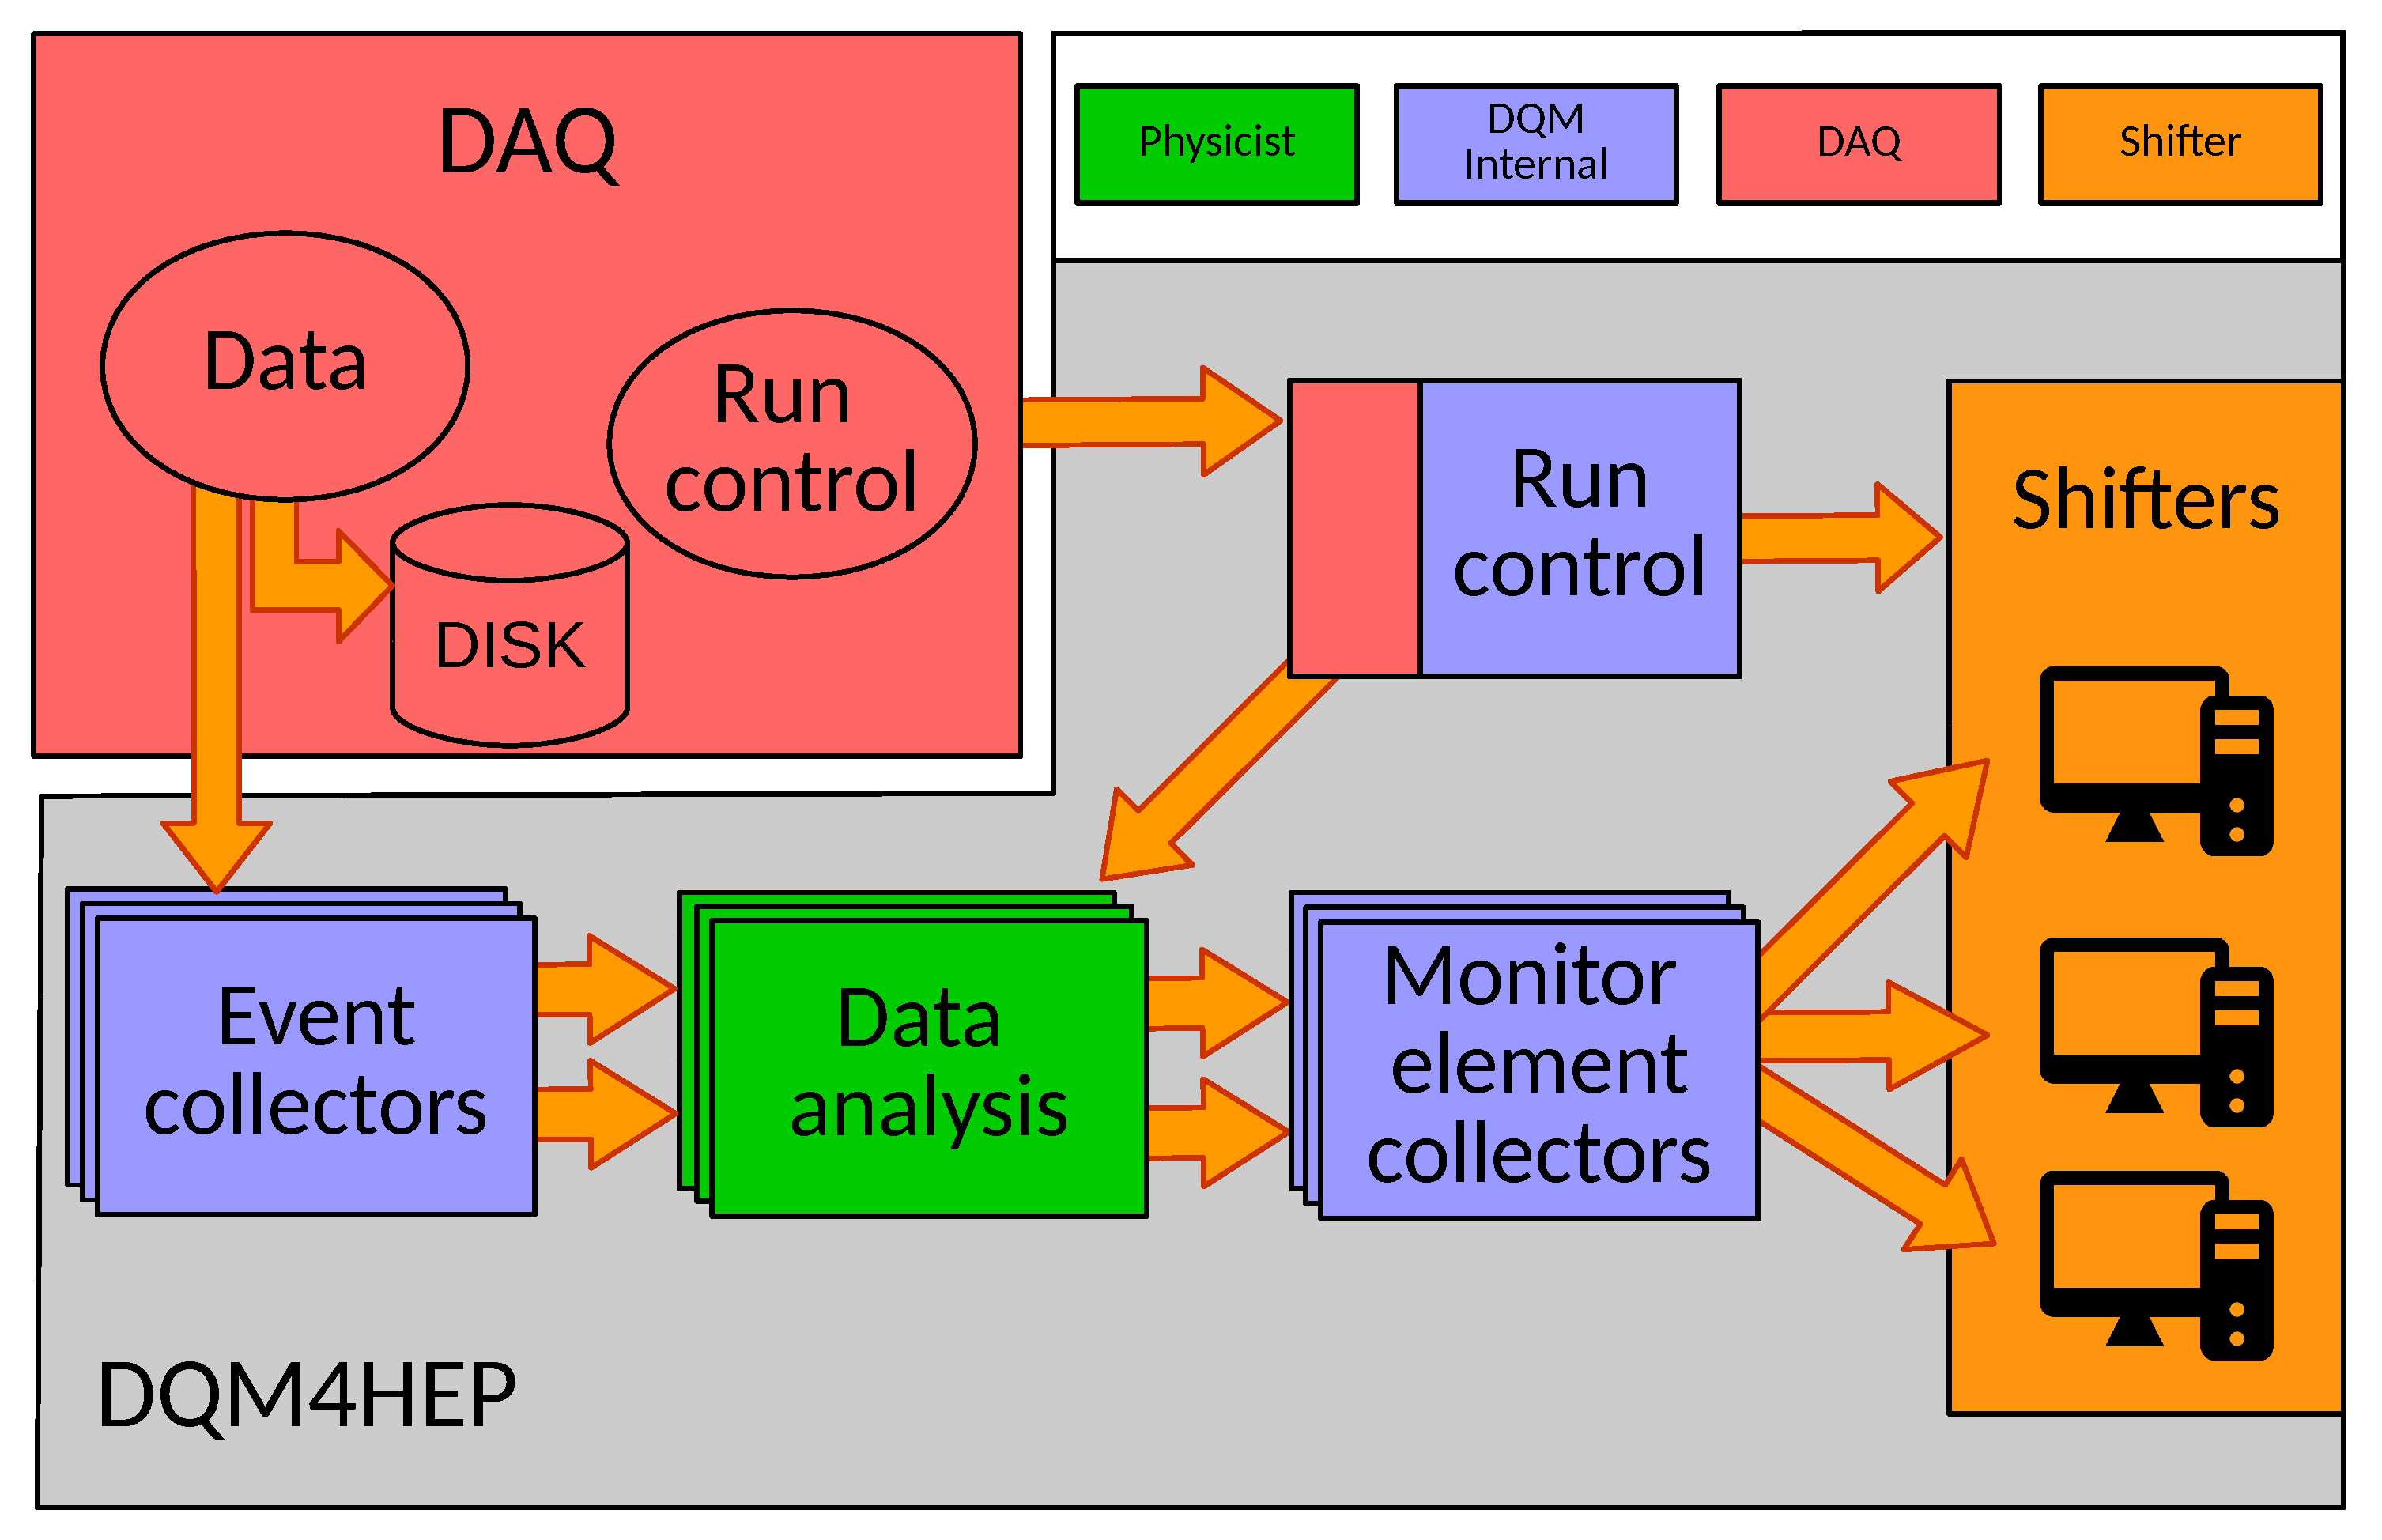
\includegraphics[width=0.95\textwidth]{../Pictures/AnalysisModuleArchitecture.pdf}
	\caption{The structure of running \acrshort{DQM4hep} online using an analysis module.}
	\label{figure:daq/dqm4hep/analysis-module}
\end{figure}

\subsubsection{Analysis modules}
Analysis modules receive events from the data acquisition system, processing the data according to a user-specified procedure to create ROOT TObjects like histograms, graphs, plots, etc. The analysis module then handles encapsulating these objects as monitor elements, and sending them to the rest of the framework for display and storage. 

An analysis module is specific to one use case, and is intended to be written by the user with their data format and processing needs in mind. However, the framework provides both templates and examples for how to write an analysis module. 

An example of the structure of the framework utilising an analysis module can be seen in Fig. \ref{figure:daq/dqm4hep/analysis-module}.

\subsubsection{Standalone modules}
Standalone modules are identical in form to analysis modules described above. The distinction is that a standalone module does not operate on data coming from the data acquisition device. One of the intended and most common usages of standalone modules is as a slow control, taking data from monitoring sensors on the device rather than data, to report on the condition of the hardware. Standalone modules could also be used to \emph{generate} data, if needed, acting as a programmed signal generator or random number generator. 

An example of the structure of the framework utilising a standalone module can be seen in Fig. \ref{figure:daq/dqm4hep/standalone-module}.

\subsubsection{File reader plugins}
A file reader is a type of plugin that reads a file from the disk and packs it into a data structure necessary for usage within \acrshort{DQM4hep}. They are used primarily for offline monitoring or data processing. File readers can be made for any kind of file, provided the user understands the data structure. There are existing examples of file readers for data stored as binary, plain text, \acrshort{LCIO} files, and ROOT TTrees. 

An example of the structure of the framework utilising a file reader plugin can be seen in Fig. \ref{figure:daq/dqm4hep/file-reader}.

\begin{figure}[p]
	\centering
	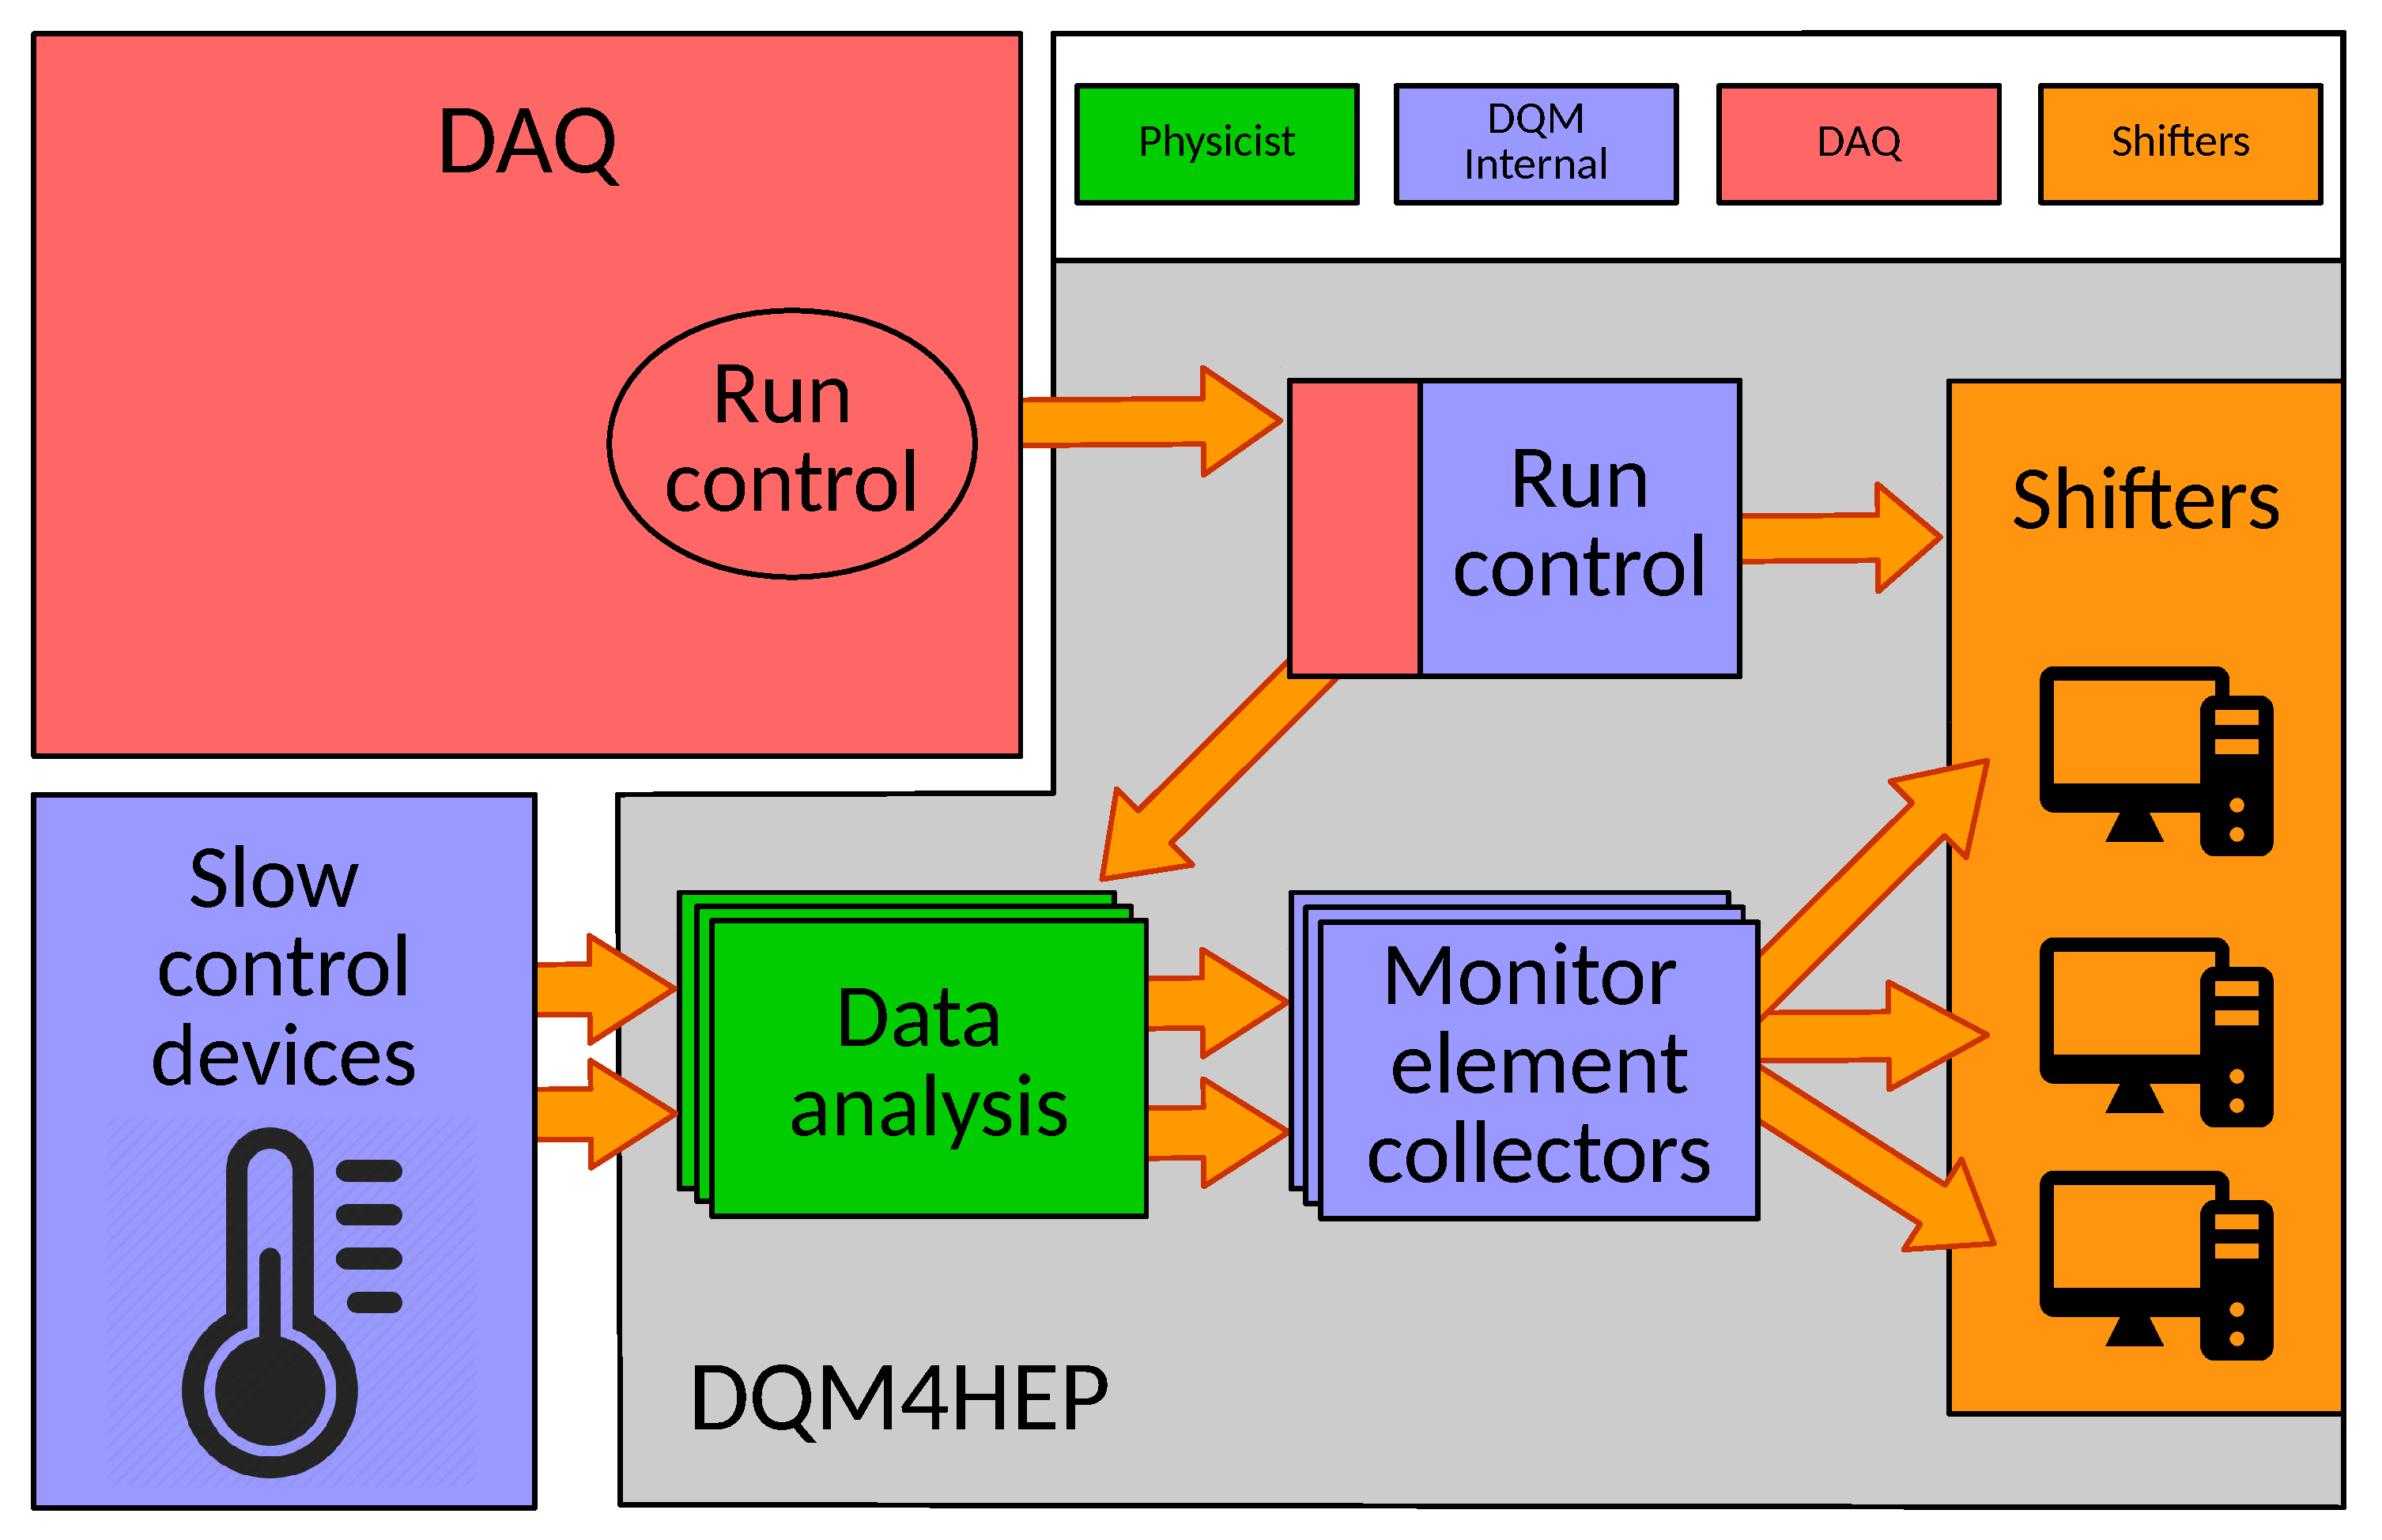
\includegraphics[width=0.95\textwidth]{../Pictures/StandaloneModuleArchitecture.pdf}
	\caption{The structure of running \acrshort{DQM4hep} online using a stand alone module.}
	\label{figure:daq/dqm4hep/standalone-module}
\end{figure}

\begin{figure}[p]
	\centering
	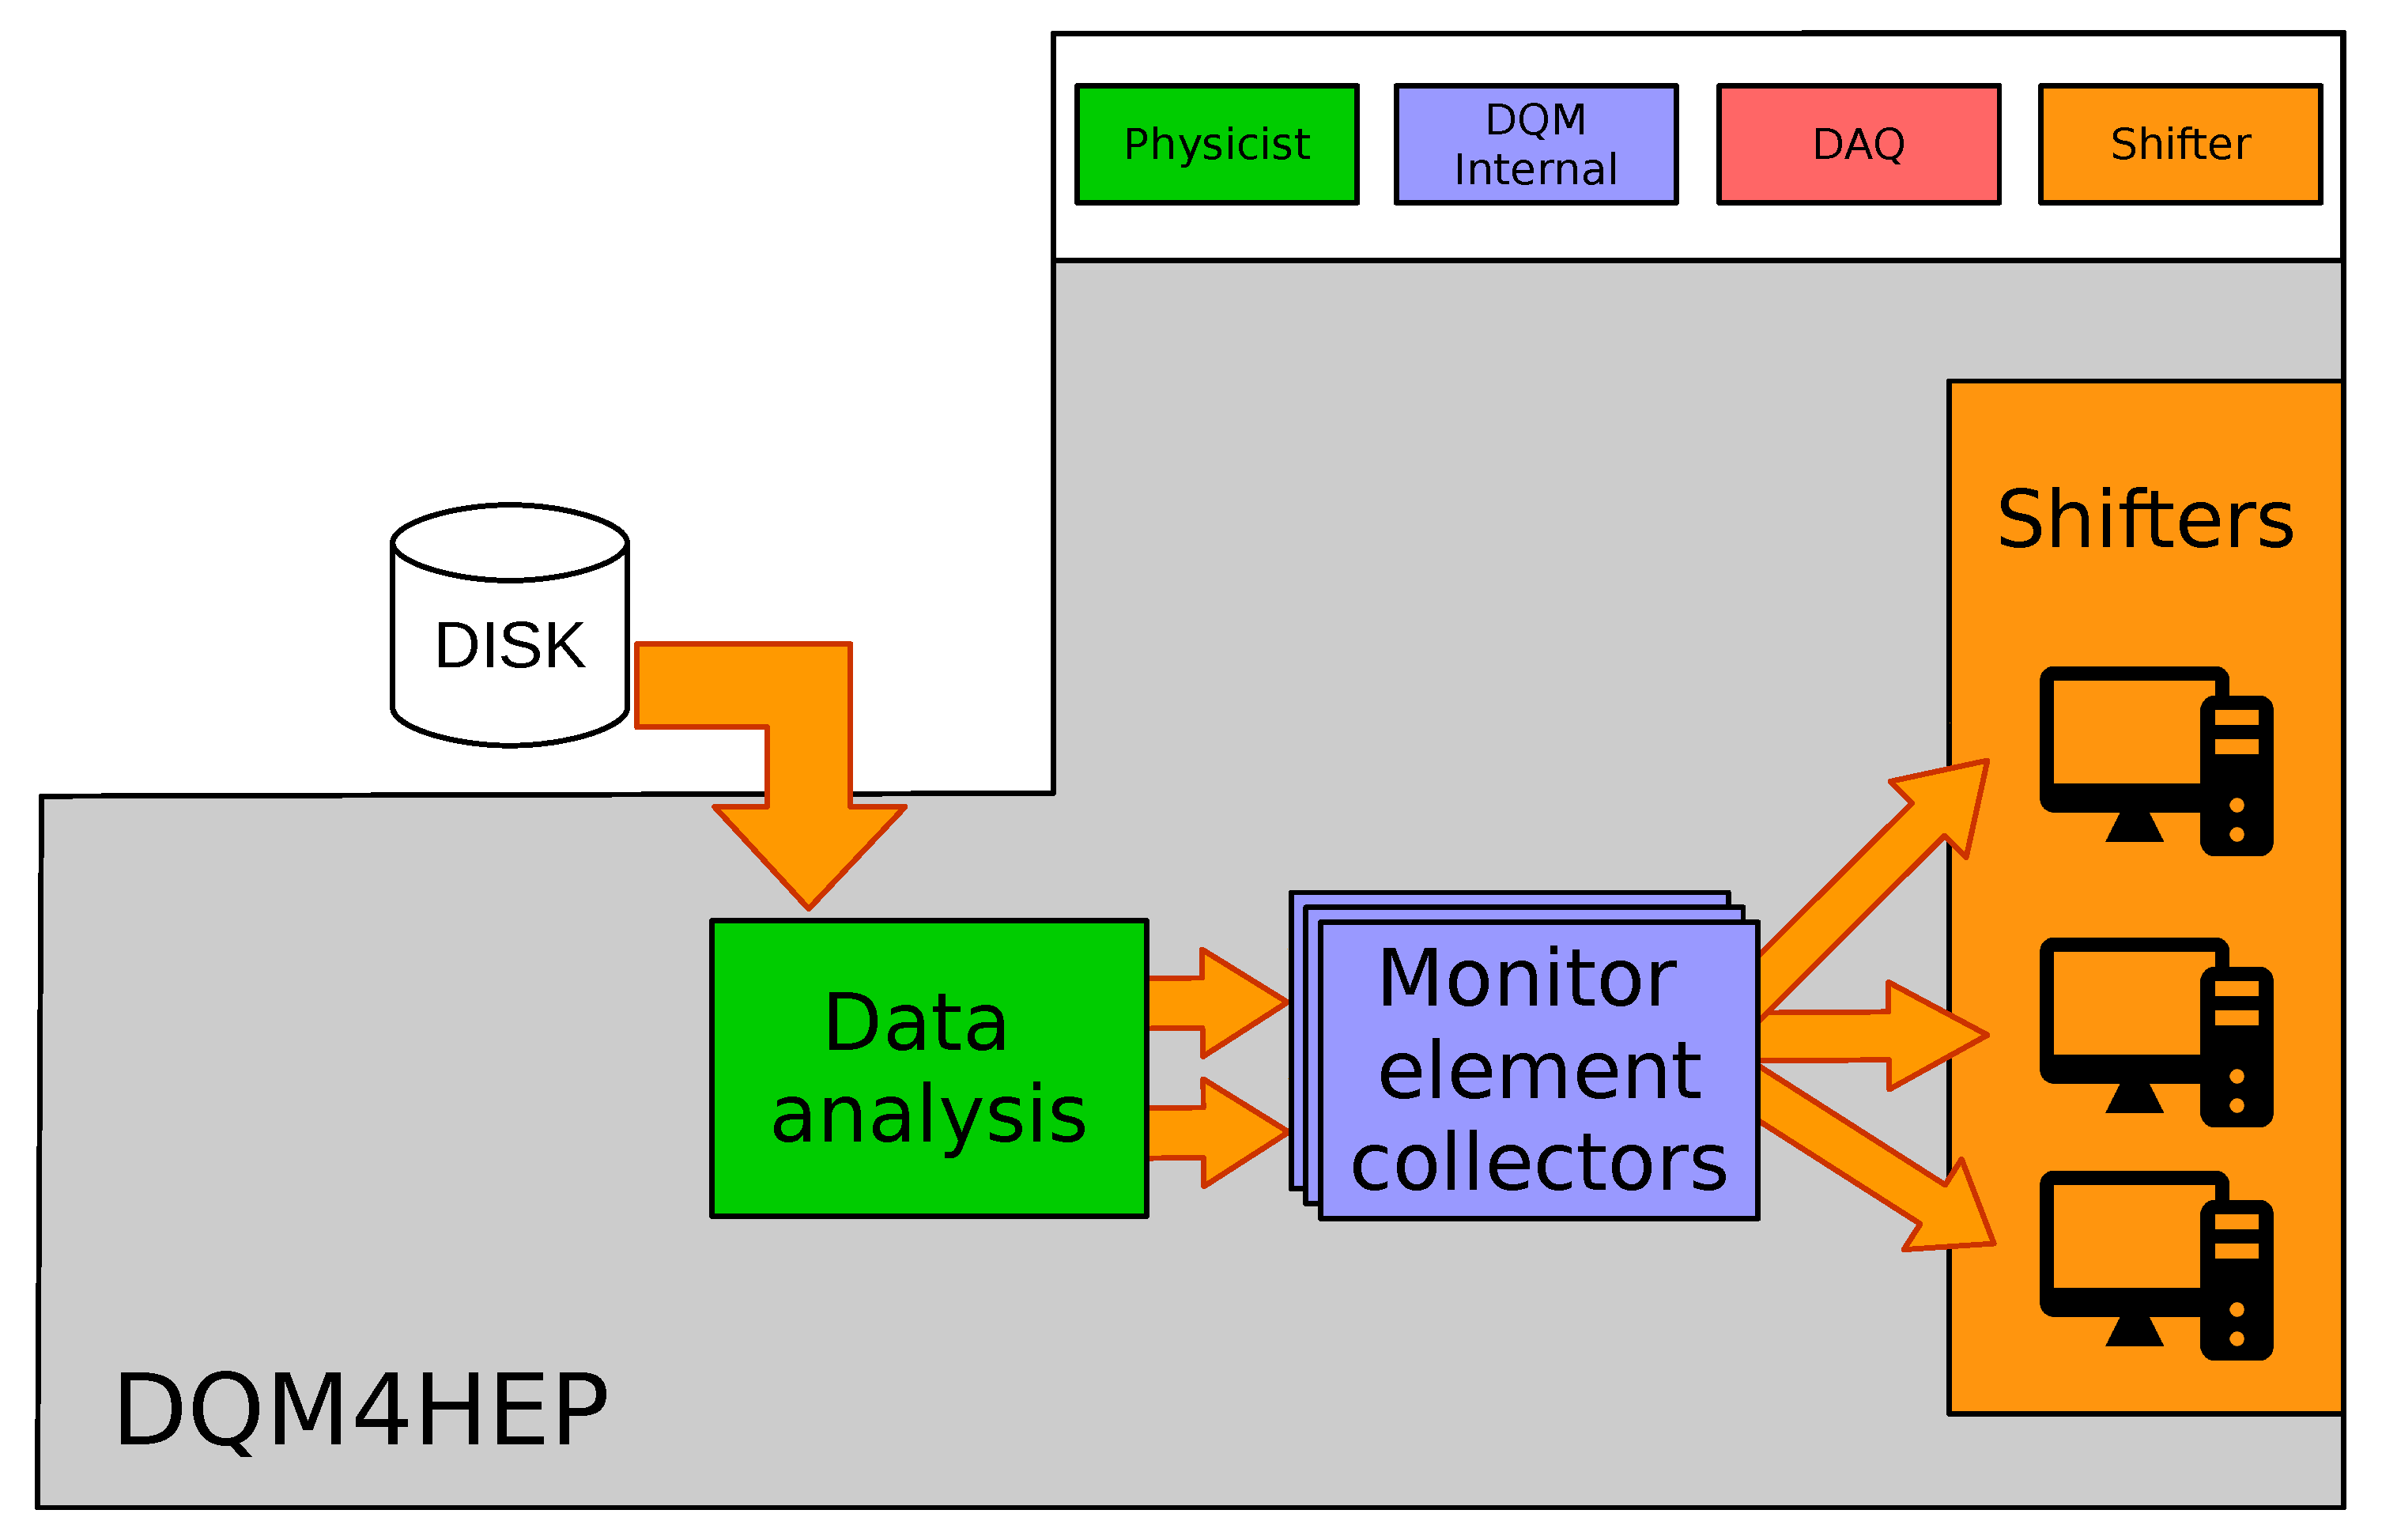
\includegraphics[width=0.95\textwidth]{../Pictures/FileReaderModuleArchitecture.pdf}
	\caption{The structure of running \acrshort{DQM4hep} offline using a file reader module.}
	\label{figure:daq/dqm4hep/file-reader}
\end{figure}

\subsubsection{File streamer plugins}
A file streamer is a type of plugin that reads data from a stream and packs it into a data structure necessary for usage within \acrshort{DQM4hep}. They are for receiving data from a data acquisition device for online monitoring. File streamers can be made for any kind of data stream, provided the user understands the data structure. File streamers are considered the ``default'' in \acrshort{DQM4hep}.

\subsection{Visualisation and graphical user interface}
As of writing, the graphic user interface (\acrshort{GUI}) and visualisation elements of the framework are still under active development for a new version. Therefore this topic will be split into two sections: one to describe the existing \acrshort{GUI}, and one to discuss the motivations and goals for the new \acrshort{GUI} under development. 

\subsubsection{Current GUI and visualisation} 
The current version of the \acrshort{GUI} is built with Qt, a free and open-source toolkit and framework for creating graphic user interfaces and widgets that are independent of the operating system. The motivation for choosing Qt was that ROOT provides an option for integration between ROOT and Qt, allowing ROOT classes like \texttt{TCanvas} to be ``embedded'' into Qt widgets. This simplified the implementation of a \acrshort{GUI}, allowing a graphical interface based on Qt to be written, then graphics from ROOT simply opened within the existing widgets and windows. % We should cite this; this information is from here: (https://root.cern.ch/root/html534/guides/users-guide/ROOTandQt.html). 

This interface is used in multiple places, including the run control process and the monitoring \acrshort{GUI}. The monitoring \acrshort{GUI} is built on a system of canvases. Each canvas can have multiple plots open, which can be resized, maximised, minimised, etc. and manipulated as normal for ROOT plots. The user can also create new canvases for more space to arrange plots.

In addition to this, there is an optional provision for a monitoring steering file, which contains presets of canvases, and the plots displayed on them. This is extremely useful when dealing with large datasets or large numbers of plots, as the plots required by the user can be opened automatically when the monitoring interface is run.

An example of the Qt-based monitoring \acrshort{GUI} in use can be seen in Fig. \ref{figure:daq/dqm4hep/old-gui}. 

\begin{figure}[h]
	\centering
	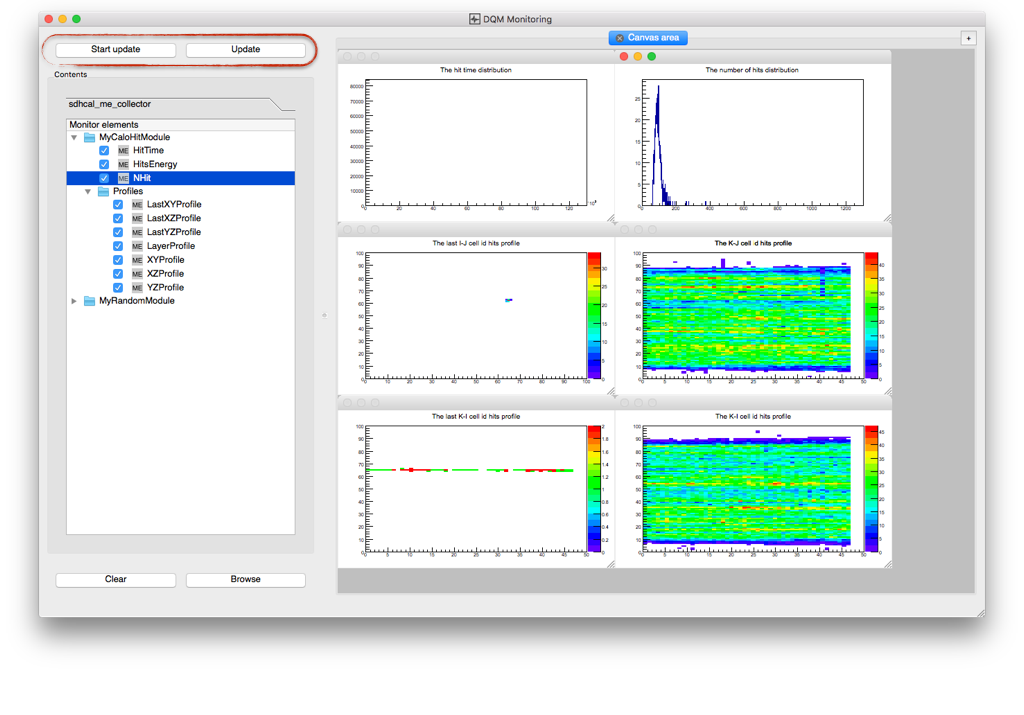
\includegraphics[width=1.0\textwidth]{../Pictures/DQM4hepMonitoringGui.png}
	\caption{An example of the current Qt-based monitoring \acrshort{GUI} in use. The panel on the left shows a list of all running analysis modules, and the monitor elements that they contain shown in a folder- or filesystem-like structure. The large right panel is the main canvas, where plots are displayed and can be resized, maximised, or manipulated as normal for ROOT objects. The data used for this demonstration is from an \acrshort{SDHCAL} testbeam.}
	\label{figure:daq/dqm4hep/old-gui}
\end{figure}

\subsubsection{New user interface and visualisation package}
For the newer versions of \acrshort{DQM4hep}, the decision was made to overhaul the \acrshort{GUI} and visualisation packages, removing Qt from the framework and moving to a web-based interface.

The removal of Qt was motivated by two reasons. Firstly, the integration with ROOT provided some complications, since running \acrshort{DQM4hep}'s Qt-based \acrshort{GUI} requires an installation of ROOT compiled with the \texttt{--enable-Qt} flag enabled. The majority of ROOT installations in remotely-accessible file systems based at \acrshort{CERN} and \acrshort{DESY} (which are heavily used for analysis and testbeams) were not compiled this way. Secondly, Qt was an additional dependency that must be installed prior to use, making the software more dependent upon the operating system, compiler tools, and environment of the machine, and thus less generic and easy to use. % Also isn't Qt support getting removed from ROOT soon? We'd need a citation for that though.

The removal of the Qt \acrshort{GUI} allows for greater freedom with development. The intended goal is to have a browser-based GUI, removing dependency on any external \acrshort{GUI} libraries and allowing it to function on any device. This will also make it more user-friendly and convenient, as the interfaces for run control, networking, and data monitoring and quality display can be simply run in different tabs of a web browser.

As of writing, the web interface is under active development by R\'{e}mi Et\'{e} and is not yet complete. However, a mock-up of the web interface can be seen in Fig. \ref{figure:daq/dqm4hep/future-gui}.

\begin{figure}[h]
	\centering
	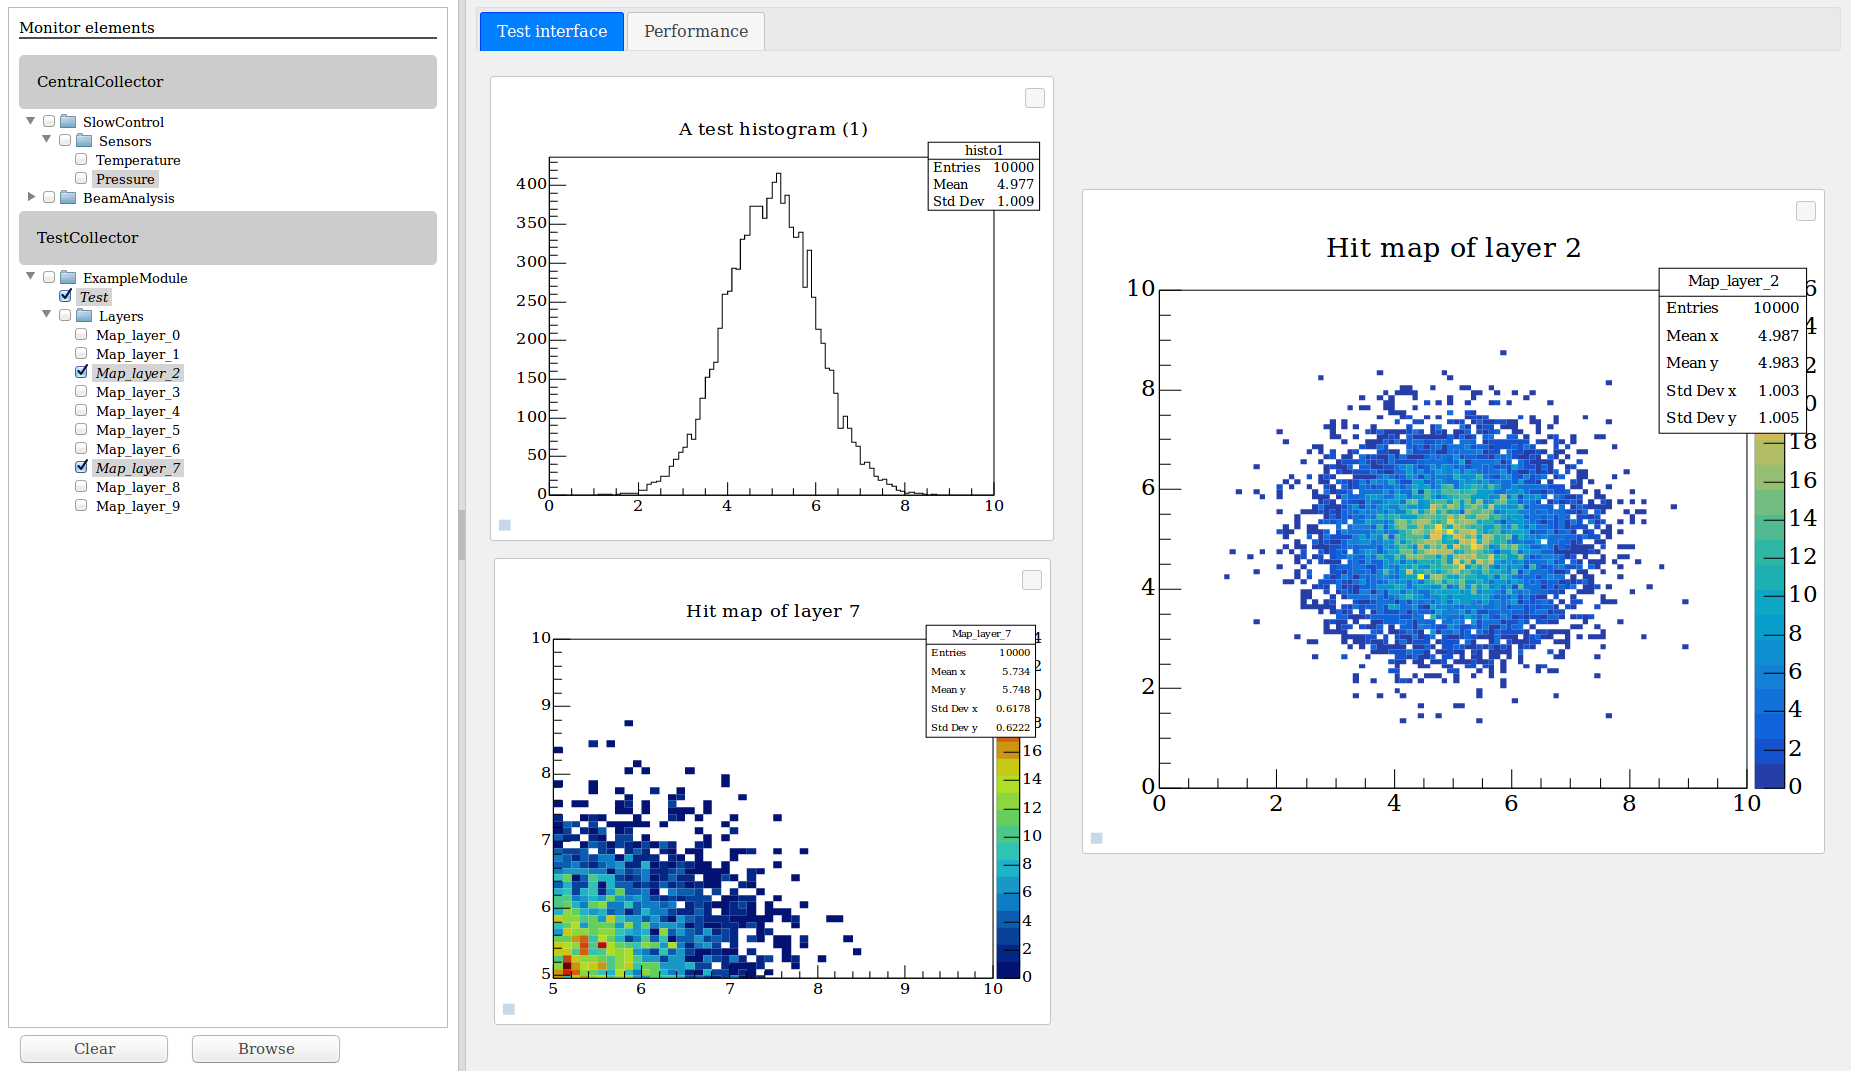
\includegraphics[width=1.0\textwidth]{../Pictures/ScreenshotWebMonitoring.png}
	\caption{A preview of the planned web-based monitoring interface. The structure is similar to the existing interface (see Fig. \ref{figure:daq/dqm4hep/old-gui}), but rendered in a web browser. The plots displayed here are not real data, but ``dummy'' data for testing purposes.}
	\label{figure:daq/dqm4hep/future-gui}
\end{figure}

\section{Analysis modules}
An analysis module is a plugin that uses data to create monitor elements, which are the core object that drives online monitoring in \acrshort{DQM4hep}. Analysis modules are thus a central piece of using \acrshort{DQM4hep} as an online monitor.

Mechanically, analysis modules are plugins that read events from a file reader or file streamer plugin, perform some user-defined process to the data to produce a plot, graph, histogram or other ROOT object before emitting it to the rest of the framework as a monitor element.

The most basic analysis module will simply structure information coming from the data acquisition device into a human-readable plot, but analysis modules are able to do anything that can be done in C++ or ROOT, so can contain an arbitrary amount of processing. This means that analysis modules can also be used for online analysis or processing of data, making them very powerful tools for online monitoring. 

\subsection{Running an analysis module}
The \texttt{dqm4hep-start-module} executable is used to run an analysis module, in combination with an XML steering file. The available arguments are as follows:

\begin{lstlisting}
-h
--help
\end{lstlisting}

Displays usage information, then exits.

\begin{lstlisting}
-f
--steering-file
\end{lstlisting}

(Required) Gives the path to the XML steering file that defines what analysis modules to run and their parameters. See the section below (need link) for more information on these steering files. 

\begin{lstlisting}
-t
--type
\end{lstlisting}

The type of module to run. This overwrites the module type in the steering file.

\begin{lstlisting}
-n
--name
\end{lstlisting}

The name for this instance of the module. This overwrites the module name in the steering file.

\begin{lstlisting}
-v
--verbosity
\end{lstlisting}

The verbosity of the logger. Options are \texttt{trace}, \texttt{debug}, \texttt{info}, \texttt{warning}, \texttt{error}, \texttt{critical}, and \texttt{off}. This is \texttt{warning} by default.

\begin{lstlisting}
--
--ignore-rest
\end{lstlisting}

Ignores any arguments following this flag.

\begin{lstlisting}
--version
\end{lstlisting}

Displays version information, then exits.

\subsubsection{Steering files}
An \acrshort{XML} steering file is used to pass parameters to the analysis module, including the type of analysis module, the plots to create, and what other processes to connect to. %An example steering file can be found in the \texttt{dqm4hep-example/tests/} directory.

Steering files are broadly made of four sections: the application settings, the archiver settings, the analysis module, and the monitor elements.

The application settings specify how to run the application itself, including which other file readers or streamers to connect to, which run control is being used, etc. 

The archiver setting specify whether the results of running the analysis module are written to an archive, which is a ROOT file containing the monitor elements that the analysis module created.

The analysis module section sets the type of analysis module to run, and gives it a unique name to distinguish it from other instances of the same module. Both of these parameters can be set at the command line (see above).

The monitor element section specifies the monitor elements used in the file. Monitor elements is a general name for any kind of ROOT object, which may be a histogram, graph, plot, drawing, etc. The name, directory, and properties of monitor elements are set here, depending on what type of object the monitor element is.

\subsection{Creating analysis modules}
%The \acrshort{DQM4hep} pages on Github have a repository to accompany this documentation – the \texttt{dqm4hep-example} package is available here\refthis. This package contains all of the tools necessary to immediately begin writing and compiling analysis modules for an existing installation of \acrshort{DQM4hep}. 

%It is recommended to fork this repository before starting, so git and Github's version control features can be used to back up code.

This sections describes the process of writing new analysis modules. begin writing and compiling analysis modules for an existing installation of \acrshort{DQM4hep}. 

In addition to writing the analysis module code, a compiled analysis module needs to be declared as a plugin for \acrshort{DQM4hep} to be able to use it. The absolute path to the library file for new analysis modules needs to be appended to the \texttt{DQM4hep\textunderscore PLUGIN\textunderscore DLL} environment variable. 

\subsubsection{Writing analysis modules}
Analysis modules must be written specifically for the type of data they receive and for a certain analysis or set of analyses to perform. This means that the ideal person to write an analysis module is someone familiar with both the experiment's event structure and the goals of the monitoring.

Each analysis module is a single .cc file. E.g. \texttt{ExampleModule.cc} would define an analysis module called \textit{ExampleModule} that would be found in the \texttt{dqm4hep-exampleproject/source/src/plugins} directory.

The .cc file then has several sections that must be written, described in separate sections below.

\subsubsection{Variable declaration}
In this section of the file, the variables that must be persistent over the entire running of the module are declared. These variables will not go out of scope, so are usually reserved for the monitor elements themselves, or counters that must persist over the entire module. Monitor elements must be declared as the \texttt{online::OnlineElementPtr} type. None of the declared variables are initialised here; initialision is done in later functions.

\subsubsection{readsettings}
This function reads the settings from the XML steering file, meaning that anything that needs to be initialised from the steering file is done here. This notably includes all monitor elements. Typically the \texttt{core::OnlineElementPtr} will have been declared during the (preamble), then is assigned here based on the steering file using the \texttt{online::ModuleApi::getMonitorElement()} function. 

\subsubsection{initModule}
This process is run once, when the analysis module is initialised. Anything that needs to be done only once at the beginning should be done here. The use of this function is limited, as most tasks that need to be reset are reset at the beginning of a run using \texttt{startOfRun()} below.

\subsubsection{startOfRun}
The \texttt{startOfRun} function handles code that should be executed only once per run, at the beginning. This is commonly used for counters that must persist over the entire run, for instance if a detector can give an error signal, a counter to store the number of error signals is initialised here so that it is persistent over the entire run, and the number of error signals can be totalled at the end of the run.

%\subsubsection{startOfCycle}

%\subsubsection{endOfCycle}

\subsubsection{endOfRun}
This is the end-of-run counterpart to \texttt{startOfRun()}. In general, this function will encapsulate logic that must deal with counters or procedures that were initialised or begun in \texttt{startOfRun()}.

\subsubsection{endModule}
This function is called when the module ends, and is usually used for deleting or cleaning up any objects created during the \texttt{initModule()} function. Most normal use cases will not need this function, as cleanup of objects such as variables or monitor elements is handled by the framework.

\subsubsection{process}
This is the function where the analysis module performs the main processing of data. In this function, events are loaded into memory from the event stream or file reader, and made available for use. Data can then be processed using normal C++ methods, then filled into monitor elements to be sent to the monitor element collectors so they can be presented in the user interface, or stored by the archiver.

\subsubsection{Plugin declaration}
Analysis modules are \acrshort{DQM4hep} plugins, so must be declared as a plugin using \acrshort{DQM4hep}'s facility for this so that the main executables can access them. At the end of the module, the following code must be included to declare the analysis module as a plugin:

\begin{lstlisting}
DQM_PLUGIN_DECL(ModuleName, "ModuleName");
\end{lstlisting}

This should take place at the very end of the file but within the \texttt{dqm4hep} and \texttt{example} namespaces.

When an analysis module is declared as a plugin, the main \acrshort{DQM4hep} executable must be given the directory of the library to load the plugin at runtime. This is done by appending the director of the library to the \texttt{DQM4hep\textunderscore PLUGIN\textunderscore DLL} environment variable:

\begin{lstlisting}
export DQM4hep_PLUGIN_DLL=$DQM4hep_PLUGIN_DLL:/path/to/module/lib/libDQMExample.so
\end{lstlisting}

Once this is added, \acrshort{DQM4hep} can access the libraries and run the analysis module.

\subsection{SimpleModule – a worked example} 
To explain the process of creating and writing analysis modules in more detail, a worked example is presented. For this we imagine a simplified particle physics detector, and write an analysis module called \texttt{SimpleModule.cc} to monitor data from it. We also write a steering file called \texttt{simple-test.xml} to run the analysis module. Each function of the analysis module will be described in depth, explaining in detail what the code is doing. 

In this example, the built-in GenericEvent event type is used. For more information on the GenericEvent type, see \cite{dqm4hep-user-manual-genericevent}. We will not be using the \texttt{startOfCycle} and \texttt{endOfCycle} functions.

%The full version of these files can be found in the dqm4hep-example repository, available here \refthis .

\subsubsection{Detector}
We can imagine a simplified particle physics detector as a square plane split into 36 tiles (6 on each side). When a hit occurs the detector reads out the location, \acrshort{ADC}, and time of the hit. Each event will correspond to a single hit.

The data acquisition device sends us an event made of four integer values:

\begin{itemize}
	\item xPos -- the position of a hit on the x-axis of the detector, from 0 to 5
	\item yPos -- the position of a hit on the y-axis of the detector, from 0 to 5
	\item ADC -- the \acrshort{ADC} of the hit, in arbitrary units, between 0 and 1500
	\item timeHit -- the time the hit occurred, in arbitrary units
\end{itemize}

\subsubsection{Goals}
Before writing the module, the variables and properties to monitor must be determined. For this detector and its analysis module, there are three goals:

\begin{itemize}
	\item Spectrum histogram -- a single histogram containing the \acrshort{ADC} of each hit for the entire run, producing an energy spectrum.
	\item Hitmap -- a hitmap showing the distribution of hits across the detector.
	\item Radiation damage -- if we imagine that \acrshort{ADC}s higher than 1000 are likely to cause radiation damage to the detector, then monitoring the number of hits in the entire run exceeding this threshold allows an estimation of how damaged the detector may be.
\end{itemize}

\subsubsection{Preamble}
Here the pointers for all monitor elements are initialised. One is required for the \acrshort{ADC} spectrum, and one for the hitmap. They don't need to have their type declared here -- this is done later. The standard style for \acrshort{DQM4hep} is to prefix all monitor element pointers with \texttt{m\textunderscore p} to distinguish them, as they are an important type.

Variables for handling the information about radiation damage are also created here, as they need to persist between events. These are declared here and will be initialised later.

\begin{lstlisting}
private:
  online::OnlineElementPtr m_pSpectrum;
  online::OnlineElementPtr m_pHitmap;
  int radiationDamageADCThreshold;
  int damageHitsCounter;
\end{lstlisting}

\subsubsection{readSettings}
Here the monitor elements are assigned, reading in their information from the \acrshort{XML} steering file. To do this the \texttt{online::ModuleApi::getMonitorElement()} function is used, which searches in the \acrshort{XML} steering file for the corresponding information. This function has three arguments: the first is always \texttt{this}, the second is the directory the monitor element is in, and the third is a string of the name given to the monitor element in the steering file. These monitor elements are placed at the top directory, so the second argument is \texttt{/}.

\begin{lstlisting}
void SimpleModule::initModule() {
  m_pSpectrum = online:ModuleApi::getMonitorElement(this, "/", "ADC_Spectrum");
  m_pHitmap   = online:ModuleApi::getMonitorElement(this, "/", "Hitmap");
}
\end{lstlisting}

Any other variables that need to be initialised only when the module starts should be placed here. This is a good place to define the threshold for radiation damage:

\begin{lstlisting}
  radiationDamageADCThreshold = 1000;
\end{lstlisting}

\subsubsection{startOfRun}
The only thing necessary to do at the start of each new run is to ensure that the counter for hits above the threshold for radiation damage is reset to zero:

\begin{lstlisting}
void SimpleModule::startOfRun(core::Run &/*run*/) {
    damageHitsCounter = 0;
}
\end{lstlisting}

This ensures that even with multiple runs in the same file, the counter resets correctly.

\subsubsection{endOfRun}
Once a run has finished, the number of hits that might have caused radiation damage should be read out. There are many ways to do this, but the simplest is to send a message to the logger:

\begin{lstlisting}
void SimpleModule::endOfRun(const core::Run &/*run*/) {
    dqm_info("Number of hits above radiation damage threshold: {0}", damageHitsCounter);
}
\end{lstlisting}

For more information on the \texttt{dqm\textunderscore info()} function and it's syntax, see the section on the logging tools here \cite{dqm4hep-user-manual-coretools}.

\subsubsection{process}
The first thing to do is make sure that the \texttt{process()} function has access to the GenericEvent. This is done by making it an argument of the function, calling it \texttt{pEvent} to make it clear that this is a pointer to an event and not an event object. Basic error-checking is then done, to ensure that the current event exists:

\begin{lstlisting}
void SimpleModule::process(core::EventPtr pEvent) {

  if (nullptr == pEvent) {
    dqm_warning("Event pointer is invalid - skipping this event");
    return;
  }
\end{lstlisting}

The \texttt{dqm\textunderscore warning()} function publishes a message to the logger, with the \texttt{warning} level. See the section on the logging tools for more information.

Forcing this function to \texttt{return} ensures that the an analysis module doesn't attempt to access an event that does not exist. Otherwise, this would cause a segmentation fault and crash the analysis module. Since the \texttt{process()} function runs separately for each event, this has the effect of skipping to the next event.

Now the pointer of the event needs to be assigned so that the object itself can be accessed. A new variable of type \texttt{core::GenericEvent} is created, then the \texttt{getEvent()} function is used to assign it.

\begin{lstlisting}
  core::GenericEvent *pGenericEvent = pEvent->getEvent<core::GenericEvent>();
\end{lstlisting}

A variable is needed to store the information pulled from the event, then the information can be extracted using the \texttt{getValues()} function:

\begin{lstlisting}
  int xPos;
  int yPos;
  int ADC;
  int timeHit;

  pGenericEvent->getValues("xPos", xPos);
  pGenericEvent->getValues("yPos", yPos);
  pGenericEvent->getValues("ADC", ADC);
  pGenericEvent->getValues("timeHit", timeHit);
\end{lstlisting}

The \texttt{getValues()} function takes two arguments: the first is a key in the form of a string, which identifies a piece of data within the GenericEvent. The second is the object to place the retrieved data into. In this case, the same names are used for simplicity. This works because the first variable is a string, used as a key to find information within the GenericEvent.

Now all the data is loaded into memory and available for use. 

First the ADC is added to the \texttt{ADC\textunderscore Spectrum} plot. To do this, the monitor element \texttt{m\textunderscore pSpectrum} must be cast to the correct ROOT object type, using the \texttt{objectTo()} function, then use ROOT's \texttt{Fill()} function:

\begin{lstlisting}
  m_pSpectrum->objectTo<TH1I>()->Fill(ADC);
\end{lstlisting}

Then the same must be done for the hitmap. This time it needs to be cast to a TH2I object and filled with the x- and y-positions as well as the \acrshort{ADC}:

\begin{lstlisting}
  m_pHitmap->objectTo<TH2I>()->Fill(xPos, yPos, ADC);
\end{lstlisting}

And lastly, a check is performed for whether the \acrshort{ADC} was high enough to cause radiation damage, and if so increment the counter:

\begin{lstlisting}
  if (ADC >= radiationDamageADCThreshold) {
    damageHitsCounter++;
  }
\end{lstlisting}

\subsubsection{Steering file}
Now the analysis module is complete, there needs to be a steering file to run it. This is started by making a file called \texttt{simple-test.xml}. Then the \texttt{<dqm4hep>} environment is opened, as this will contain everything else:

\begin{lstlisting}
<dqm4hep>

    <!-- everything else will be in here -->

</dqm4hep>
\end{lstlisting}

There are then four sections to write: the application settings, the archiver settings, the analysis module, and the monitor elements.

\subsubsection{Application settings}
This section of the steering file controls the parameters that are needed to run the module itself. This part of the file is where the module is specified to be running online (receiving events from an event collector) or offline (receiving events from a file reader).

This analysis module will be run offline, so the important fields here are \texttt{EventReader}, which is which type of file reader to use to read events, and \texttt{EventFileName}, which specifies the path to the file to read.

If this were running online, the \texttt{RunControl}, \texttt{EventCollector}, \texttt{EventSource} and \texttt{MonitorElementCollector} would have to give the names of those processes. When running offline, these names can be set to anything, so they are given dummy names.

\begin{lstlisting}
<settings mode="EventReader">
  <parameter name="EnableStatistics"> true </parameter>
  <parameter name="EventReader"> SimpleEventReader </parameter>
  <parameter name="EventFileName"> /foo/bar/simpleEventDatafile.root </parameter>
  <parameter name="CyclePeriod"> 1 </parameter>
  <parameter name="CycleCounter"> 0 </parameter>
  <parameter name="CycleTimeout"> 0 </parameter>
  <parameter name="RunControl"> DummyRunControl </parameter>
  <parameter name="EventCollector"> DummyEventCollector </parameter>
  <parameter name="EventSource"> DummyEventSource </parameter>
  <parameter name="MonitorElementCollector"> DummyMECollector </parameter>
</settings>
\end{lstlisting}

\subsubsection{Archiver settings}
This section controls the archiver, which creates an archive of all monitor elements in the form of a ROOT file when the analysis module exits. If the archiver isn't needed, it can be set to \texttt{enable="false"} and ignored.

In this case the archiver is needed, so it is set to \texttt{true}. A filename for the archive needs to be given, e.g. \texttt{archive-run42.root}. The OpenMode is chosen to be \texttt{RECREATE} as the archive should be re-written every time the module is run, although \texttt{APPEND} would add events onto an existing file. \texttt{AllowOverwrite} is set to \texttt{true} so that old archives can be overwritten easily. As run numbers are not used in the analysis module, \texttt{AppendRunNumber} is set to \texttt{false}.

\begin{lstlisting}
<archiver enable="true">
  <parameter name="FileName" value="archive-run42.root"/>
  <parameter name="OpenMode" value="RECREATE"/>
  <parameter name="AllowOverwrite" value="true"/>
  <parameter name="AppendRunNumber" value="false"/>
  <selectors>
    <selector regex=".*" select="true"/>
  </selectors>
</archiver>
\end{lstlisting}

\subsubsection{Analysis module}
This section contains a declaration of which analysis module to execute, and the name to give it. A running analysis module needs a unique name to distinguish it from other modules of the same type running in the same environment.

This steering file has to run SimpleModule. Only one instance is needed at a time, but the name has to be different than the module's base name, so:

\begin{lstlisting}
<module type="SimpleModule" name="mySimpleModule"/>
\end{lstlisting}

\subsubsection{Monitor elements}
This section is where the monitor elements to use and the parameters of the ROOT objects are declared. This entire section will be within the \texttt{<storage>} and \texttt{<monitorElements>} environments:

\begin{lstlisting}
<storage>
  <monitorElements>

    <!-- monitor elements will go here -->

  </monitorElements>
</storage>
\end{lstlisting}

To create a ROOT object, the \texttt{<bookElement>} environment is used to declare it's type, path, name, title, and any other parameters the ROOT object requires. For example, to create a histogram for the \acrshort{ADC} spectrum, a TH1I is needed as the \acrshort{ADC}s are integers. The range of the \acrshort{ADC}s is from 0 to 1500, so the range can be set accordingly.

\begin{lstlisting}
<bookElement type="TH1I" path="/" name="ADC_Spectrum" title="Spectrum of all ADCs" nBinsX="150" minX="0" maxX="1500">
</bookElement>
\end{lstlisting}

Similarly, the monitor element for the hitmap is defined:

\begin{lstlisting}
<bookElement type="TH2D" path="/" name="Hitmap" title="Hitmap of the example detector" nBinsX="6" minX="0" maxX="5" nBinsY="6" minY="0" maxY="5">
</bookElement>
\end{lstlisting}

\subsubsection{XML loops}
In this example, loops aren't necessary, but defining monitor elements using a for-loop in \acrshort{XML} is a useful feature, so it is discussed here. For example, if one of the goals were to create a histogram for each of the 36 tiles in the detector, a for-loop would allow this to be created with a smaller amount of code

To do this, the \texttt{<for>} environment is used, using \texttt{tileNumber} as the id. Then a template monitor element definition is written out using \texttt{\$ FOR{tileNumber}} whenever the tile number should be inserted:

\begin{lstlisting}
<for id="tileNumber" begin="0" end="35" increment="1">
  <bookElement type="TH1D" path="/" name="Tile$FOR{channelNum}" title="Spectrum for tile $FOR{channelNum}" nBinsX="150" minX="0" maxX="1500">
  </bookElement>
</for>
\end{lstlisting}

This would then create a series of monitor elements called \texttt{Tile0}, \texttt{Tile1}, \texttt{Tile2}, etc.

\subsubsection{Building and running}
To compile the analysis file, the normal build commands are issued from the \texttt{dqm4hep-example/build} directory:

\begin{lstlisting}
cmake ..
make install
\end{lstlisting}

Running cmake is only needed for the first compilation after creating a new module – it isn't necessary when recompiling a module that has been compiled before.

Once the analysis module has compiled successfully, \acrshort{DQM4hep} must be given the path to its libraries so that the main installation of \acrshort{DQM4hep} can utilise it. This is done by appending the path to the libraries to the \texttt{DQM4hep\textunderscore PLUGIN\textunderscore DLL} environment variable:

\begin{lstlisting}
export DQM4hep_PLUGIN_DLL=$DQM4hep_PLUGIN_DLL:/path/to/dqm4hep-example/lib/libDQMExample.so
\end{lstlisting}

In order to run, the network manager dim must also be running, but for offline use this is simple. In a new terminal window:

\begin{lstlisting}
export DIM_DNS_NODE=localhost
dns
\end{lstlisting}

Then to run the analysis module, the \texttt{dqm4hep-start-module} executable is run, pointing it to the steering file using the \texttt{-f} argument. Since a logging output at the `info` level was implemented, the argument \texttt{-v} must be given to manually set the logging level to \texttt{info} so that it can be seen in the output.

\begin{lstlisting}
dqm4hep-start-module -f simple-test.xml -v info
\end{lstlisting}

The analysis module will then run. Once it has finished, the archiver will create the archive in the directory it was run in.

\section{Data quality monitoring}
Data quality monitoring (\acrshort{DQM}) is a type of data monitoring where the data is tested using some form of statistical or mathematical process to produce a value corresponding to the ``quality'' of the dataset. This can take many forms, such as comparing an experimental dataset to reference data acquired from previous experiments, or requiring that the $\chi^2$ or p-value of a dataset may need to pass a certain threshold to be considered valid.

The definition of the ``quality'' statistic will differ according to a variety of factors such as the type of data, the aim of an experiment, etc. Common examples are p-values, or binary pass-fail tests where data that passes has a quality of 1, and 0 otherwise.

One of the benefits of data quality monitoring is that it provides a more reproducible and robust set of checks on data-taking, allowing quantitative analysis of the performance of a detector prototype. It can also be used as a way for shifters without detailed knowledge of the hardware, software, or physics to determine whether the detector is performing as intended during a testbeam when experts are not available, by using the quality statistics as a guide.

Previous versions of \acrshort{DQM4hep} did not have infrastructure to support data quality monitoring, but this was added during refactoring in preparation for the next release version. Once this was in place, this permitted an array of quality tests to be developed, implemented, and tested. 

A quality test (or \acrshort{qtest}) processes a series of monitor elements (ROOT TObjects) according to a set of criteria defined in the test's code. This test produces a numerical result between 0 and 1, referred to as the ``quality''. Within the framework, quality tests are self-contained C++ code files, which hook into the framework's system for execution. Quality tests are run by using the executable \texttt{dqm4hep-run-qtests} and a steering file to define parameters, such as which files to load, which quality tests to execute, and what the passing and failing boundaries are for each quality test. 

\subsection{Quality tests}
The quality tests that have been implemented in \acrshort{DQM4hep} are described in detail below. Each test requires a certain type of object as an input and has it's own definition of what the ``quality'' statistic represents. Some quality tests also require a reference to compare against the input data, which is also described.

A summary of the quality tests can be found in Table \ref{table:dqm4hep/qtests}.

\subsubsection{Property within expected test}
\label{sec:property-qtest}
This is a quality test that takes either a TH1 or TGraph object, and finds some user-defined parameter. The parameter must be one of: mean, mean90, root mean square (RMS), root mean square 90 (RMS90), or median. It then checks whether either: that this parameter is within a user-specified range; or that it is above or below the user-specified threshold. If a range is being used, the result is the p-value of the property being within the specified range. If a threshold is being used, then the result is 1 if the property passes the threshold, 0 otherwise.

\subsubsection{Exact reference comparison test}
This is a quality test that takes any TObject, and compares it to a user-specified reference object (which must be of the same type). The result is 1 if the two objects are exactly identical, 0 otherwise. 

\subsubsection{Fit parameter in range test}
This is a quality test that takes either a TH1, TGraph, or TGraph2D object and plots a user-defined function onto it, solving for one of the parameters of the function, then checks it against a user-defined range. The result is the p-value of the parameter being within the specified range.

\subsubsection{Kolmogorov-Smirnov test}
This is a quality test that takes either a TH1 or a TGraph object, and performs the Kolmogorov-Smirnov test between that object and a specified reference. The result is the p-value of the Kolmogorov-Smirnov test. The Kolmogorov-Smirnov test is intended for unbinned data, not histograms, but ROOT provides a function for performing the Kolmogorov-Smirnov test on histograms, so this is functionality is also included for the sake of completeness.

\subsubsection{Pearson $\chi^2$ test} % We should probably cite the Pearson chi^2 test itself
This is a quality test that takes a TH1 object and performs the Pearson $\chi^2$ test between that object and a specified reference. This test is analogous to the Kolmogorov-Smirnov test, but is designed specifically to work for binned histogram data. The result is the p-value output by the $\chi^2$ test. 

\begin{table}[htp]
\centering
	\begin{tabular}{ l l l l } 
	\hline \hline 
	\textbf{Quality Test} & \textbf{TObjects} & \textbf{Required} & \textbf{Optional} \\ \hline

	PropertyWithinExpectedTest & TH1 & Property & \\
	 & TGraph & Method &  \\
	 &  & (see \ref{sec:property-qtest}) &  \\ \hline

	ExactRefCompareTest & Any TObject & None & CompareUnderflow\\
	 &  &  & CompareOverflow \\ \hline
	
	FitParamInRangeTest & TH1 & FitFormula, & GuessParameters \\
	 & TGraph & TestParameter & FunctionRange \\
	 & TGraph2D & DeviationLower & UseLogLikelihood \\
	 &  & DeviationUpper & UsePearsonChi2 \\
	 &  &  & ImproveFitResult \\ \hline
	
	KolmogorovTest & TH1 & None & UseUnderflow \\
	 & TGraph &  & UseOverflow \\ \hline
	
	Chi2Test & TH1 & None & ComparisonType \\
	 &  &  & UseUnderflow \\
	 &  &  & UseOverflow \\ \hline \hline

	\end{tabular}
	\caption{Table summarising all quality tests implemented in \acrshort{DQM4hep} and their properties.}
	\label{table:dqm4hep/qtests}
\end{table}

\subsection{Running quality tests}
Quality tests can be run using the \texttt{dqm4hep-run-qtests} executable, found in \texttt{dqm4hep-core/bin/}. This executable handles the running of the actual binaries for each \acrshort{qtest}, as well as obtaining monitor elements from the ROOT file and the setting of parameters. This executable has one required arguments and several optional ones, detailed below. 

\subsubsection{Arguments}

\begin{lstlisting}
-h
--help
\end{lstlisting}

Displays usage information, then exits.

\begin{lstlisting}
-i <string>
--input-qtest-file <string>
\end{lstlisting}

(Required) Gives the path to the \acrshort{XML} steering file that defines what quality tests to run, their parameters, and what monitor elements to run them on. See the section below for more information on these steering files.

\begin{lstlisting}
-c
--compress-json
\end{lstlisting}

Turns on compression for the \acrshort{JSON} \acrshort{qtest} report output file. Off by default.

\begin{lstlisting}
-w
--write-monitor-elements
\end{lstlisting}

Turns on writing of monitor elements in the \acrshort{qtest} report. Off by default.

\begin{lstlisting}
-p <string>
--print-only <string>
\end{lstlisting}

Prints only the quality reports of the given flag. Options are \texttt{undefined}, \texttt{invalid}, \texttt{insuf\textunderscore stat}, \texttt{success}, \texttt{warning}, \texttt{error}.

\begin{lstlisting}
-e <string>
--exit-on <string>
\end{lstlisting}

Forces the program to exit if any \acrshort{qtest} results in the given code. or greater. Options are \texttt{ignore}, \texttt{failure}, \texttt{warning}, \texttt{error}. This is \texttt{failure} by default.

\begin{lstlisting}
-v <string>
--verbosity <string>
\end{lstlisting}

The verbosity of the logger. Options are \texttt{trace}, \texttt{debug}, \texttt{info}, \texttt{warning}, \texttt{error}, \texttt{critical}, and \texttt{off}. This is \texttt{warning} by default.

\begin{lstlisting}
-q <string>
--qreport-file <string>
\end{lstlisting}

Gives the path of the \acrshort{qtest} report output file (in \acrshort{JSON}) format.

\begin{lstlisting}
-o <string>
--root-output <string>
\end{lstlisting}

Gives the path of a ROOT output file to save the processed monitor elements.

\begin{lstlisting}
--
--ignore_rest
\end{lstlisting}

Ignores any arguments following this flag.

\begin{lstlisting}
--version
\end{lstlisting}

Displays version information, then exits.

\subsubsection{Steering file}
Steering files use \acrshort{XML} to store all the information needed to execute a \acrshort{qtest}. An example steering file can be found in \texttt{dqm4hep-core/tests/test \textunderscore samples.xml}.

There are two main sections: the \texttt{<qtests>} block and the \texttt{<monitorElements>} block, both of which must be within the \texttt{<dqm4hep>} XML tag.

The \texttt{<qtests>} block defines the \acrshort{qtest}s to execute along with their settings or parameters, without reference to what they will be run on. The structure and parameters of these is highly dependent upon the \acrshort{qtest} being used – see the section for each \acrshort{qtest} above.

The \texttt{<monitorElements>} block opens a file using the \texttt{<file>} tag, within which each monitor element is opened with \texttt{<fileElement>}. Inside this tag, all of the \acrshort{qtest}s to execute on this monitor element are given. In this example below, the \acrshort{qtest}s \texttt{ExampleTest1} and \texttt{ExampleTest2} are both performed on the monitor element \texttt{TestHistogram}:

\begin{lstlisting}[language=XML]
<monitorElements>

  <file name="test_samples.root">
    <fileElement path="\TestDirectory" name="TestHistogram">
    <qtest name="ExampleTest1" />
    <qtest name="ExampleTest2" />
    </fileElement>
  </file>

</monitorElements>
\end{lstlisting}

Some kinds of \acrshort{qtest}s require reference objects to compare against, which must be declared in the \texttt{<references>} block. References have a \texttt{name} parameter which gives the path to the file used as a reference, and an \texttt{id} which is a short tag for referring to them later in the XML file. For example:

\begin{lstlisting}[language=XML]
<references>
  <file id="mc-ref" name="montecarlo_reference_samples.root"/>
  <file id="ex-ref" name="experiment_reference_samples.root"/>
</references>
\end{lstlisting}

When a \acrshort{qtest} that requires a reference is declared, the reference is given within the \texttt{<fileElement>} tag:

\begin{lstlisting}[language=XML]
<fileElement path="\TestDirectory" name="TestHistogram">
  <reference id="MyReference"/>
  <qtest name="ExampleTest1"/>
</fileElement>
\end{lstlisting}

This performs the \acrshort{qtest} \texttt{ExampleTest1} on the monitor element \texttt{TestHistogram}, looking for another ROOT object of the same name within the file \texttt{MyReference} points to. It is also possible to use a specific object in a file as the reference:

\begin{lstlisting}[language=XML]
<fileElement path="\TestDirectory" name="TestHistogram">
  <reference id="MyReference" path="/path/to/the/reference/file" name="ReferenceHistogram"/>
  <qtest name="ExampleTest2"/>
</fileElement>
\end{lstlisting}

In this case, this performs \texttt{ExampleTest2} on the monitor element \texttt{TestHistogram}, using the object \texttt{ReferenceHistogram} as the reference. 

\subsection{Writing quality tests}
Users can create their own quality tests if the included tests do not satisfy their requirements. Quality tests are a type of plugin – see the \textit{plugin system} section of the \acrshort{DQM4hep} documentation \cite{dqm4hep-user-manual-plugins} for more information on plugins, including how to write and compile them.

The code for the built-in quality tests can be found in \texttt{dqm4hep-core/source/src/plugins/} and can be used as references or templates. Files for quality tests should be given a descriptive name in CamelCase, and end with \texttt{Test}, e.g. \texttt{ExactRefCompareTest.cc}.

The code for a quality test requires only a single .cc file, which has four functions: the constructor, the destructor, readSettings, and userRun. Each is discussed in a separate subsection below. If required, further functions can be implemented as needed. This is left for the user to decide.

Code should be written to catch common errors and throw appropriate exceptions, especially for errors that cause segmentation faults. This will help to avoid a \acrshort{qtest} preventing other \acrshort{qtest}s from running should an error occur. Errors are reported using the \texttt{report.m\_message()} function, and the error message will appear in the summary of the \acrshort{qtest} after it has run.

\subsubsection{Constructor and destructor}
For the constructor and destructor, it's enough to copy existing code, changing the name of the \acrshort{qtest} and the variables to be initialised. The program that runs \acrshort{qtest}s handles everything else. Care should be taken to initialise variables properly and to give the \acrshort{qtest} a good description:

\begin{lstlisting}[language=C++]
ExampleTest::ExampleTest(const std::string &qname)
    : QualityTest("ExampleTest", qname),
      m_someFloatParameter(0.f),
      m_someIntParameter(0)
{
  m_description = "A description of the test's functionality, as well as the meaning of the quality statistic it outputs.";
}
\end{lstlisting}

\subsubsection{readSettings}
The \texttt{readSettings} function initialises the variables of the \acrshort{qtest} from the \acrshort{XML} steering file, which is loaded into memory via \texttt{xmlHandle}. This function should be used to read in information from the \acrshort{XML} file and validate it to make sure the test can be run. Variables are read in using a combination of pre-processor macros and XmlHelper. For example:

\begin{lstlisting}[language=C++]
RETURN_RESULT_IF(STATUS_CODE_SUCCESS, !=, XmlHelper::readParameter(xmlHandle, "PropertyName", m_property))
\end{lstlisting}

Note that the above example will fail if the parameter is not present in the XML file, so should only be used for parameters that are required. If a parameter is optional, use the \texttt{RETURN\_RESULT\_IF\_AND\_IF} macro instead. This allows the parameter to be returned if it is found, or does nothing if it is not. For example:

\begin{lstlisting}[language=C++]
    RETURN_RESULT_IF_AND_IF(STATUS_CODE_SUCCESS, STATUS_CODE_NOT_FOUND, !=, XmlHelper::readParameter(xmlHandle, "PropertyName", m_property))
\end{lstlisting}

For more information on status codes, pre-processor macros, and \acrshort{XML} parsing with XmlHelper, see the core tools section of the documentation.

Parameters should be checked to make sure that the \acrshort{qtest} can be run and that the result is meaningful. While \texttt{XmlHelper::readParameter} and similar functions can take an optional fourth argument for a validator delta function, users should make code clear and readable by using \texttt{if-else} statements. This is especially important when checking against more complicated criteria.

\subsubsection{userRun}
The \texttt{userRun} function defines the process of the \acrshort{qtest} itself, using the monitor element. The result \textit{must} be a float between 0.0 and 1.0 that represents the ``quality'' or ``goodness'' of the test. The meaning of this quality statistic depends on the test but is often a p-value. At absolute minimum, it should represent a pass-fail case, so that a passing \acrshort{qtest} gives a quality of 1 and a failing \acrshort{qtest} gives a quality of 0.

The monitor element must first be cast to an appropriate class. This should be done using the \texttt{objectTo} function. For example, if the monitor element is a TH1:

\begin{lstlisting}[language=C++]
TH1* myHistogram = pMonitorElement->objectTo<TH1>();
\end{lstlisting}

After this, the object can be accessed using it's normal methods, and the \acrshort{qtest} can be written using normal C++ code for ROOT objects.

It is useful to include a check for whether the monitor element exists and is the correct type, to prevent segmentation faults, using a comparison to \texttt{nullptr} and throwing an appropriate status code if the check fails. For example:

\begin{lstlisting}[language=C++]
if (nullptr == pMonitorElement->objectTo<TH1>())
{
  report.m_message("Object does not exist or is of unrecognised type!");
  throw StatusCodeException(STATUS_CODE_INVALID_PTR);
}
\end{lstlisting}

The meaning of these status codes is documented under \textit{Status codes and useful preprocessor macros} in the core tools section of the documentation.

Once the quality statistic of the test is known, it is output using \texttt{report.m\_quality}. Any other information can be output using \texttt{report.m\_message} – this is useful for including comments on the result.

\section{Documentation and user manual} 
One of the biggest hurdles for the promotion and uptake of a new framework is the lack of understanding or familiarity with it's use. Many research teams will continue to use existing software solutions, which may be suboptimal or difficult to use, according to the principle of ``better the devil you know than the devil you don't''. The first step to overcoming this is to produce clear, readable and complete documentation across the entire range of features the framework has.

The \acrshort{DQM4hep} framework has two sets of documentation with different intended readers and different aims, so these will be discussed separately.

\subsection{Doxygen documentation}
Doxygen is a tool for automatically generating documentation resources for C++ code, relying on marked sections of documentation written within the actual code itself. Doxygen is able to directly obtain the structure of code, objects, functions, etc. from the code, allowing it to automatically generate a complex and rich set of documentation that categorises and indexes objects based on their inheritance, namespace, etc.

Doxygen can also generate an HTML- or \LaTeX -based document that can be used as a local reference guide or hosted online. This makes Doxygen a powerful tool for documenting the technical aspects of code, demonstrating hierarchies of functions and objects, and an extremely useful reference guide for large programs or frameworks.

While Doxygen documentation is extremely useful, it does have some limitations. Doxygen functions more as a technical reference for code, lacking any overviews or instructions due to it's automatic generation. This kind of documentation lacks a holistic element, and has no way for new users or those less familiar with the codebase to understand the overarching concepts. This can make it inaccessible for new users. The way this was addressed will be discussed in the next section.

DQM4hep has a Doxygen website hosted on the internet, which is available here\cite{dqm4hep-doxygen}.

\subsection{User manual} % include elements of the documentation and overview of how to use program as a whole; examples of use.
The existing documentation featured the common elements of the framework -- such as the plugin system, event interface, logger, and XML parser -- explained in detail, with clear examples and straightforward advice on their use.

My contribution to this was to write in-depth explanations on the structure, usage, and creation of analysis modules and quality tests, the two parts that are most specific to end-users. The experience acquired using the framework and deploying it on testbeams for the first time, as well as integrating it with different detectors, provided a strong knowledge base to write the user manual intended for a user approaching the framework for the first time. These testbeams are described in more detail in Chapters \ref{chapter:aidatestbeams} and \ref{chapter:ideatestbeam}.

The user manual can be found online here\cite{dqm4hep-user-manual}.

\subsubsection*{Analysis module guide}
There is an in-depth explanation of each of the component functions of an analysis module, discussing which actions or data processing should be done in each, and their intended purposes. There is also an explanation of the \acrshort{XML} steering files that are necessary to run an analysis module, and instructions on how the executable is run, along with it's arguments.

In addition to this there is a worked example of an analysis module from start to finish. A simplified particle physics detector and it's data format is defined, and then the reader is lead through the process of writing an analysis module step-by-step and function-by-function to obtain certain plots and results from the data. This is intended to give a more concrete demonstration of usage, as an easier to follow example. This section is also written in simple and plain English in order to be as accessible as possible.

%Along with this documentation there is the \texttt{dqm4hep-example} Github repository [cite], which contains all of the code used in the analysis module user manuals, as well as the required cmake and make files to begin compiling projects right away. The intention of this repository is for new users to make a copy, write their own modules, and have everything needed for compiling and running them ``out of the box'' straight away. The user manual references this repository, so that users can see the files from the worked example in their full form.

\subsubsection*{Quality testing guide}
There is extensive documentation of quality testing; each quality test is described in detail, including their purpose, output, required parameters, and optional parameters. In addition to this, there is a guide for how to run quality tests, including an explanation of running from the command line and an in-depth look at the structure of the \acrshort{XML} steering files required.

Finally there is a section explaining how to write new quality tests. This includes a detailed explanation of the purpose of each function within a quality test file, what the required outputs are and how to utilise them, error testing, and advice on maintaining a style consistent with the rest of the framework.

\section{Adaptation to other detectors}
Due to the modularity and genericness of \acrshort{DQM4hep}, the process of deploying it for a new detector is simple -- the only parts of \acrshort{DQM4hep} that need to be made for any specific use case are the analysis modules, standalone modules, streamer plugin, and file reader plugin. For all of these plugins, there are templates available in the codebase, as well as examples of in-use plugins for other detectors. A few special \acrshort{DQM4hep}-specific functions are necessary for these plugins to hook into the framework properly, but apart from these all user-provided plugins are written in normal C++ code that also integrates ROOT, so should be familiar to most users.

A file streamer or file reader must be written by the user given a specific data structure. This requires knowledge of both the event data model of the data acquisition setup, as well as the structure of the data files. The ideal person to write this code is someone with detailed knowledge of the data acquisition software being used, and the data storage or streaming. 

In general, only one of the file streamer or file reader plugins will be needed. Both of these plugins are similar in structure and differ only on where they get the data from -- a file reader loads a file from disk, whereas a streamer loads it from the data acquisition system. If the data will be monitored offline or ``nearly-online'' by loading files from disk, then a file reader plugin must be written. If the data is to be monitored online, then a streamer plugin must be written. 

Once the information is accessible from either the file reader or streamer, the framework handles passing this data to the analysis modules. Analysis modules are a type of plugin which take data that has been packaged into events by a file reader or streamer plugin and performs some analysis on it. The main action an analysis module must do is create a monitor element (a ROOT TObject) then emit it to the rest of the framework. Before this step an arbitrary amount of processing can be done, e.g. checking validation bits, thresholds, error-checking, and so on. Monitoring the data quality can be done from within analysis modules but this is not recommended as dedicated quality tests (see section above) are available.

For each analysis module that is being run, an \acrshort{XML} steering file is required to provide the parameters and networking information to all the processes needed. A single steering file can call only a single analysis or standalone module, but multiple steering files can be run in parallel by the framework.

Examples of using \acrshort{DQM4hep} with testbeams both within the \acrshort{AIDA}-2020 community and outside of it can be found in Chapters \ref{chapter:aidatestbeams} and \ref{chapter:ideatestbeam}, respectively.